\newcommand{\DoNotLoadEpstopdf}{}
\documentclass[11pt]{article}
\usepackage[margin=1in]{geometry}
\usepackage[T1]{fontenc}
\usepackage{lmodern}
\usepackage{amsmath,amssymb,amsthm,mathtools,mathrsfs}
\usepackage{microtype}
\usepackage{booktabs,array}
\usepackage{tikz}
\usetikzlibrary{arrows.meta,positioning,calc}
\usepackage[hidelinks]{hyperref}
\hypersetup{pdftitle={The first lattice correction to Bloch's law},
 pdfauthor={OpenAI},
 pdfsubject={Low-temperature spontaneous magnetization of the three-dimensional quantum Heisenberg ferromagnet}}
\ifdefined\pdftrailerid\pdftrailerid{}\fi
\ifdefined\pdfsuppressptexinfo\pdfsuppressptexinfo=15\fi
\numberwithin{equation}{section}
\allowdisplaybreaks[2]
\setlength{\emergencystretch}{2em}
\setcounter{tocdepth}{1}
\newtheorem{theorem}{Theorem}[section]
\newtheorem{proposition}[theorem]{Proposition}
\newtheorem{lemma}[theorem]{Lemma}
\newtheorem{corollary}[theorem]{Corollary}
\newtheorem{claim}[theorem]{Claim}
\theoremstyle{definition}
\newtheorem{definition}[theorem]{Definition}
\theoremstyle{remark}
\newtheorem{remark}[theorem]{Remark}
\newcommand{\R}{\mathbb R}
\newcommand{\Z}{\mathbb Z}
\newcommand{\PP}{\mathbb P}
\newcommand{\EE}{\mathbb E}
\newcommand{\ind}{\mathbf 1}
\newcommand{\D}{\mathcal D}
\newcommand{\ip}[2]{\langle #1,#2\rangle}
\newcommand{\norm}[1]{\lVert #1\rVert}
\newcommand{\abs}[1]{\lvert #1\rvert}
\DeclareMathOperator{\Tr}{Tr}
\DeclareMathOperator{\dist}{dist}
\DeclareMathOperator{\supp}{supp}
\DeclareMathOperator{\divg}{div}
\title{The first lattice correction to Bloch's law}
\author{OpenAI}
\date{October 5, 2026}
\begin{document}
\maketitle
\begin{abstract}
We prove the first lattice correction to Bloch's law for the
three-dimensional nearest-neighbor quantum Heisenberg ferromagnet at every
fixed spin $S=\tfrac12,1,\tfrac32,\ldots$. The spontaneous-magnetization
deficit agrees with the full ideal-magnon density up to
$o(\beta^{-5/2})$. In addition to the leading Bloch term, this gives the
correction $3\zeta(5/2)(\beta S)^{-5/2}/(128\pi^{3/2})$.
The magnetization is the right derivative at zero field of the
thermodynamic pressure; the volume limit precedes the field derivative,
and the low-temperature limit is taken last.
\end{abstract}
\tableofcontents
\section{Introduction}\label{sec:introduction}

The leading low-temperature magnetization deficit of a three-dimensional
ferromagnet is determined by long-wavelength spin waves. At the next
order, the lattice dispersion becomes visible. We prove that this first
lattice correction gives the corresponding term in the spontaneous
magnetization of the quantum Heisenberg ferromagnet, for every fixed
positive half-integer spin.

\subsection{The model and the result}

Let $S\in\{\tfrac12,1,\tfrac32,\ldots\}$ and
$\Lambda_N=\{-N,\ldots,N\}^3\subset\Z^3$.
At each site $x$ let $\boldsymbol S_x=(S_x^1,S_x^2,S_x^3)$ be the
spin-$S$ operators on $\mathbb C^{2S+1}$. With free boundary conditions,
the Hamiltonian and total $z$-spin are
\[
 H_{S,N}=-\sum_{\substack{\{x,y\}\subset\Lambda_N\\ |x-y|_1=1}}
                \boldsymbol S_x\cdot\boldsymbol S_y,
 \qquad M_N=\sum_{x\in\Lambda_N}S_x^3.
\]
Every unordered lattice edge is counted once. For inverse temperature
$\beta>0$ and field $h\ge0$, define
\[
 p_{S,\beta}(h)
 =\lim_{N\to\infty}\frac1{\beta|\Lambda_N|}
             \log\Tr e^{-\beta(H_{S,N}-hM_N)},
 \qquad
 m_S(\beta)=\partial_{h+}p_{S,\beta}(0).
\]
The pressure limit is the usual finite-range thermodynamic limit.
Convexity and the bound $|M_N|\le S|\Lambda_N|$ give its finite right
derivative. Thus the volume limit precedes the zero-field limit in
the definition of $m_S$.

The full ideal-magnon density uses the lattice dispersion
$\varepsilon_S(k)=2S\sum_{j=1}^3(1-\cos k_j)$:
\begin{equation}\label{eq:ideal-density}
 n_S^{\mathrm{sw}}(\beta)
   =\int_{[-\pi,\pi]^3}
      \frac{d^3k}{(2\pi)^3\,[e^{\beta\varepsilon_S(k)}-1]}.
\end{equation}
The integral is finite in dimension three.

\begin{theorem}\label{thm:main}
For every fixed $S\in\{\tfrac12,1,\tfrac32,\ldots\}$,
\[
 \lim_{\beta\to\infty}(\beta S)^{5/2}
       \bigl[S-m_S(\beta)-n_S^{\mathrm{sw}}(\beta)\bigr]=0.
\]
\end{theorem}

Expanding the lattice heat kernel gives the following explicit form.
Here $\zeta$ denotes the Riemann zeta function.
\begin{corollary}\label{cor:expansion}
For every fixed positive half-integer $S$,
\[
 S-m_S(\beta)
 =\frac{\zeta(3/2)}{8\pi^{3/2}}(\beta S)^{-3/2}
  +\frac{3\zeta(5/2)}{128\pi^{3/2}}(\beta S)^{-5/2}
  +o\bigl((\beta S)^{-5/2}\bigr).
\]
\end{corollary}

\subsection{Historical context and inputs}

The spin-wave description of a ferromagnet begins with Bloch's prediction
of a magnetization deficit proportional to \(T^{3/2}\), where \(T=\beta^{-1}\)
\cite{Bloch1930}.  The bosonic representation of Holstein and Primakoff
made the distinction between independent spin waves and their interactions
explicit \cite{HolsteinPrimakoff1940}.  Dyson subsequently developed the
interaction expansion \cite{Dyson1956a,Dyson1956b}.  In that expansion,
the terms of orders \(T^{5/2}\) and \(T^{7/2}\) in the magnetization already
arise from the lattice dispersion of independent magnons
\cite[Section~5, Equation~(71)]{Dyson1956b}; the leading interaction
contribution is of order \(T^4\)
\cite[Section~8, Equation~(122)]{Dyson1956b}.
Later effective-field-theory calculations retain this distinction and
extend the expansion for cubic lattices \cite{Hofmann2017}.
The present result justifies the first lattice correction at fixed quantum
spin, with magnetization defined by the zero-field right derivative of the
thermodynamic pressure.

Rigorous thermodynamic estimates developed through a different sequence
of arguments.  Conlon and Solovej obtained a low-temperature free-energy
bound with the predicted power but a nonoptimal coefficient
\cite{ConlonSolovej1991}; T\'oth improved this bound using a random-stirring
representation \cite{Toth1993}.  Correggi, Giuliani, and Seiringer proved
the leading spin-wave free-energy asymptotic in three dimensions for every
fixed spin \cite[Theorem~2.1]{CGS2015}.  Their result concerns the free
energy at zero field; extracting the right derivative at zero field
requires additional control.  Benedikter obtained an interaction
correction as a free-energy upper bound in the different regime
\(S\to\infty\) with \(\beta S\) fixed \cite{Benedikter2017}.

The probabilistic framework comes from T\'oth's cycle representation for
spin \(1/2\) \cite{Toth1993} and Nachtergaele's realization of spin \(S\)
inside the symmetric tensor product of \(2S\) spin-\(1/2\) spaces
\cite[Section~2.2]{Nachtergaele1994}.
Within this framework, two companion manuscripts provide the direct inputs.
\emph{Spontaneous magnetization in the quantum Heisenberg ferromagnet}
establishes low-temperature ordering and uniform estimates for loops
conditioned to be up at prescribed points
\cite[Theorems~1.1 and~7.5]{Ordering}.
\emph{Bloch's Law for Finite-Range Heisenberg Ferromagnets in Three Dimensions}
proves the leading magnetization asymptotic and develops the return-kernel
and pressure arguments used below \cite[Theorem~1.1 and Sections~2--7]{BlochLaw}.

The heat-kernel bounds follow the energy-dissipation and composition
argument of Nash \cite[pp.~935--936]{Nash1958}, with the local geometric
and flow estimates supplied by the companions.

\subsection{The comparison behind the proof}

The cycle representation replaces a spin-$S$ site by $2S$ binary slots.
Random exchanges join the slot trajectories into cycles on a time
circle of length $\beta$. Requiring selected slot-time points to be up
is called pinning. A single-slot down probability can be expressed
through the return probability of a walk in the complement of the
cycles that avoid the pins. We recall the precise identities in
Section~\ref{sec:loops}.

The return walk sees a periodic, moving set of obstacles. It loses
an edge when the other endpoint is occupied by an obstacle, and is
transported when that obstacle exchanges with a hole. The comparison
must preserve both effects. For an isolated obstacle, their signed
contribution to the free heat equation telescopes to the change of
the profile along the obstacle trajectory, together with a cutoff error.
The resulting bound is controlled by its displacement over a short
block and smaller time-variation and cutoff terms.
This is the cancellation that improves the
error beyond the leading spin-wave scale.

We organize the proof around a finite-dimensional capacity criterion
in Section~\ref{sec:capacity}. The criterion compares a hitting
function with a trial potential and requires two estimates: a scalar
residual pairing, and a bound on the residuals against Dirichlet
energy. It applies to nonselfadjoint contraction kernels, so no
reversibility of the exposed environment is needed. The free trial
potential sums returns over all positive periods; the capacity
comparison therefore retains the full Bose sum.

Section~\ref{sec:geometry} strengthens the pin estimates to joint
snapshot bounds and proves the path and heat-kernel estimates needed
on short blocks. Section~\ref{sec:profiles} constructs the free trial
potential, and Section~\ref{sec:sources} proves the signed cancellation
and the ordered Duhamel identities. Sections~\ref{sec:scalar}
and~\ref{sec:energy} establish the two residual estimates. Finally,
Section~\ref{sec:pressure} converts the uniform pinned comparison to
the right derivative of the thermodynamic pressure and proves
Corollary~\ref{cor:expansion}.

Throughout the proof $S$ is fixed. Constants may depend on $S$;
the local comparison estimates will be uniform in volume and in the
allowed deterministic pin sets. All norms on finite slot spaces use
counting measure.

\section{Pinned cycles and the return walk}\label{sec:loops}

We first express a pinned spin deficit as a return probability for one
particle.  The resulting walk moves through a periodic set of holes.
We state precisely the loop identities and pin estimates imported from
\cite{Ordering,BlochLaw}; the estimates that improve their precision are
proved in Section~\ref{sec:geometry}.

\subsection{The picture and its pin law}

Fix a finite free-boundary cube $\Lambda=\Lambda_N\subset\Z^3$ and write
$H_{S,\Lambda}=H_{S,N}$ and $\ell=2S$.  Its slot set is
$V_\Lambda=\Lambda\times\{1,\ldots,\ell\}$.
A slot edge joins every pair of slots whose sites are nearest neighbors.
The base picture consists of independent Poisson clocks of rate $1/2$
on these undirected edges during $[0,\beta)$, and independent uniform
permutations of the $\ell$ slots at each site at the seam $0$.
Following the swaps and then the seam permutations produces directed
cycles on the time circle $\R/\beta\Z$.  A slot-time point at an
instantaneous operation is understood to lie just after that operation.
Write $\EE_{\mathrm b}$ for expectation under the base law.
This is the exchange-cycle representation of T\'oth \cite{Toth1993},
with the higher-spin symmetrization discussed by Nachtergaele
\cite[Section~2.2]{Nachtergaele1994}.

Let $\partial_{\mathrm{in}}\Lambda$ be the sites of $\Lambda$ having a
neighbor outside it, and put
\[
 D_0=\partial_{\mathrm{in}}\Lambda\times\{1,\ldots,\ell\}
                              \times(\R/\beta\Z).
\]
An \emph{allowed pin set} is $D=D_0\cup F$, where $F$ is a finite
deterministic set of slot-time points.  Pins require the corresponding
cycles to be up.  If $n_D(\omega)$ is the number of cycles missing $D$,
define
\begin{equation}\label{eq:pinlaw}
 Z_D=\EE_{\mathrm b}2^{n_D},\qquad
 \PP_D(d\omega)=Z_D^{-1}2^{n_D(\omega)}\PP_{\mathrm b}(d\omega),
 \qquad
 \mathcal B_D=\bigcup_{C\cap D=\varnothing} C.
\end{equation}
Under the associated color law, cycles meeting $D$ are up and all other
cycles are independently up or down with equal probabilities.  These
definitions also make sense for $D=\varnothing$.  We denote probabilities
under the color law by $\PP_D^{\mathrm{col}}$.

Hereafter all low-temperature bounds are uniform in the finite cube and
in its allowed deterministic pin set.  Their constants may depend on
the fixed spin and on fixed geometric constants, but not on the number
or placement of the extra pins.

\subsection{Exposure and a fresh walk}

For an allowed $E$ and an unpinned point $i$, set $P=E\cup\{i\}$.
Sample the picture under $\PP_P$ and expose all cycles in $\mathcal B_P$,
including their inter-site jumps and their seam mappings.  At each time
their occupied slots are called \emph{obstacles}; the complementary slots
are \emph{holes}.  Every pin is a hole at its prescribed time.

At fixed exposure, the fresh walk on holes has rate $1/2$ on every edge
between holes.  When an obstacle swaps into a hole, that hole is
transported in the opposite direction.  A swap of two obstacles has no
effect on the holes.  At the seam the walk uses a fresh uniform bijection
between the remaining slots at each site, respecting the exposed part of
the seam permutation.  The exposure is repeated periodically, while all
transition randomness of the walk is resampled on each turn.  This is
a time-inhomogeneous Markov walk at fixed exposure; it is not obtained
by following the unexposed part of a single conditioned picture.

Let $q_i$ be its probability, starting from $i$, of returning to the
same slot-time point at strictly positive elapsed time before hitting
$E$.  A return can occur only at an integer number of periods.  We use
$r=\EE_Pq_i$ and $d_E(i)=\PP_E^{\mathrm{col}}(i\text{ is down})$.

\begin{proposition}[Loop and pin inputs]\label{prop:loopinputs}
The following statements hold at every finite volume and $\beta>0$.
\begin{enumerate}
\item If $q_\Lambda$ is the number of slot edges and $c(\omega)$ the
number of cycles, then
\[
 \Tr e^{-\beta H_{S,\Lambda}}
       =e^{\beta q_\Lambda/4}\EE_{\mathrm b}2^{c(\omega)}.
\]
The spectral distribution of the total $z$-spin is obtained by the
unpinned color law, assigning $+1/2$ to each up slot and $-1/2$ to each
down slot at time zero.  The expectation, in this normalized color law,
of the exponential of $\beta$ times the field times this sum is the
ratio of the field and zero-field partition functions.
\item For the allowed sets $E,P$ and point $i$ above,
\begin{equation}\label{eq:pinreturn}
 \PP_E(i\in\mathcal B_E)=\frac{2r}{1+r},
 \qquad d_E(i)=\frac{r}{1+r},\qquad r=\EE_Pq_i.
\end{equation}
\item More generally, let $T$ be a nonempty finite set of points at one
deterministic time, disjoint from an allowed $D$, and put $P'=D\cup T$.
Expose $\mathcal B_{P'}$ and let $q_j^{D,T}$ be the fresh-walk probability
from $j\in T$ of hitting $T$ at positive elapsed time before $D$.  Then
\begin{equation}\label{eq:simultaneouspin}
 \PP_D(T\subset\mathcal B_D)\le (2r_T)^{|T|},
 \qquad
 r_T=\frac1{|T|}\sum_{j\in T}\EE_{P'}q_j^{D,T}.
\end{equation}
\item For any allowed $D$, the factorial measure of $j$ distinct
inter-site marks under $\PP_D$ is bounded by $2^j$ times the base
factorial measure.  This holds with chronological ordering and with
arbitrary deterministic restrictions on the edges and times.
\end{enumerate}
\end{proposition}

The first assertion is the exact spin-$S$ representation in
\cite[Proposition~2.2]{Ordering}, with the present rate and Hamiltonian
normalizations.  The second combines the one-pin weight identity and
fresh-turn identity in \cite[Propositions~2.4 and~2.8]{BlochLaw}.
The third combines \cite[Proposition~3.1 and Lemma~4.4]{Ordering}; in
particular, no spatial separation of the test points is assumed.
The last assertion is \cite[Lemma~2.4]{Ordering}.  The statements include
all-time boundary pins by the dense-boundary limit proved there.

\subsection{Kernel conventions and energy}

Kernels act forward on column vectors, with counting inner products and
norms.  Killing on a pin means a projection at its prescribed time;
boundary killing is imposed throughout, including at interval endpoints.
Killing on exit from a spatial set retains the exit rates on the
generator's diagonal.  The adjoint of an interval reverses the order of
all factors, inverts transports, transposes the seam averages, and
reverses the order of killing projections.  Thus the two sides of an
instantaneous operation remain distinct slices.  Each seam factor is
included exactly once in a traversal.

Extend the hole graph by making every slot outside $\Lambda$ available.
Its edges join available slots over neighboring sites.  For a vector
extended by zero on the inner boundary and outside $\Lambda$, define
\begin{equation}\label{eq:dirichlet}
 \D_t(v)=\frac12\sum_{\{a,b\}\text{ available at }t}
                                      (v(a)-v(b))^2.
\end{equation}
The exterior extension will allow flows to infinity; all test vectors
will have finite support.

\begin{lemma}[Contraction and energy loss]\label{lem:kernelenergy}
At fixed exposure, every killed interval kernel and its adjoint are
substochastic in both counting sums and contract counting $\ell^p$ for
$p=1,2,\infty$.  Between instantaneous operations a propagated vector
satisfies
\[
 \frac{d}{dt}\norm{v_t}_2^2=-2\D_t(v_t).
\]
The squared norm cannot increase at an instantaneous operation.

Let $U$ be a one-period kernel with any allowed pin killings, and let $y$
vanish on its cut killing slots.  Set
$e_y=\ip{y}{(I-U)y}\ge0$.  For either $U_d=U$ or $U^*$, let $Y_t$ be
the adjoint propagation of $y$ from the terminal cut to an intermediate
slice.  Then
\begin{equation}\label{eq:energy}
 \int_{\mathrm{traversal}}\D_t(Y_t)\,dt\le e_y,
 \qquad
 \norm{y-U_d^*y}_2^2\le2e_y.
\end{equation}
The contraction and local norm-loss statements hold with extra spatial
killing and for intervals continued across a period cut.
Equation~\eqref{eq:energy} concerns one complete traversal; each copy
of that traversal has the same bound.
\end{lemma}

\begin{proof}
For one realization of the fresh exchanges and seam completions, the
unkilled trajectories define a bijection between the endpoint hole sets.
Deleting trajectories that encounter a killing set gives a partial
permutation.  Averaging proves the two substochastic bounds and the
$\ell^1$ and $\ell^\infty$ contractions.  Rowwise Cauchy--Schwarz gives
the $\ell^2$ contraction, as in
\cite[Section~3.1]{BlochLaw}.  Transposition gives the stated reverse
realization and the same bounds.

On a smooth interval the generator is symmetric, with rate $1/2$ on
each available edge and Dirichlet killing rates.  Summing by edges proves
the norm-loss identity.  Zero extension gives exactly
\eqref{eq:dirichlet}: a surviving interior slot has no edge directly to
the exterior of the cube.  Instantaneous contractions can only add to
the norm loss.  Finally, for $V=U$ or $U^*$, the real quadratic forms
agree and
\[
 \norm{y}_2^2-\norm{Vy}_2^2
       =2e_y-\norm{y-Vy}_2^2.
\]
This identity, contraction, and the integrated norm loss prove
\eqref{eq:energy}.
\end{proof}

All these are finite-volume statements with piecewise smooth evolution.
We disregard the null event of coincident Poisson marks or marks at a
prescribed deterministic time.  Deterministic operations that coincide
are composed in their assigned order.  The kernels are measurable from
finite-time transition formulas, and hitting probabilities from
increasing finite-horizon limits.  Consequently we may average them
under the actual picture law, including on events defined below.

\section{A capacity comparison on one period}\label{sec:capacity}

The probability of returning to a pin includes arbitrarily many turns
of the fresh walk.  We compare this probability directly, through a
hitting problem on one cut.  The local conclusion needed for
magnetization is the following uniform comparison.  Write
$B_r(x)=\{z\in\Z^3:|z-x|_\infty\le r\}$ for a site ball and set
$R_*=\lceil\beta^{5/3}\rceil$.

\begin{proposition}[Uniform comparison away from pins]\label{prop:comparison}
For every fixed positive half-integer $S$ there are
$\beta_0(S)<\infty$ and a function $\varepsilon_S(\beta)\to0$
as $\beta\to\infty$ such that the following holds for every
$\beta\ge\beta_0(S)$.
Let $\Lambda$ be any finite cube, let $E=D_0\cup F$ with $F$ any
finite deterministic set of slot-time pins, and let $i=(x,a)$ be a
time-zero post-seam slot.  Suppose that $B_{50R_*}(x)$ is interior
to $\Lambda$ and that $E$ has no point above this ball.  Then
\begin{equation}\label{eq:pinnedcomparison}
 \abs{d_E(i)-\frac1\ell n_S^{\rm sw}(\beta)}
 \le \varepsilon_S(\beta)\beta^{-5/2}.
\end{equation}
The same uniform error bound, after enlarging $\varepsilon_S$ if
necessary, holds for
$\abs{\EE_{E\cup\{i\}}q_i-\ell^{-1}n_S^{\rm sw}(\beta)}$.
\end{proposition}

The bound is uniform over the number and locations of all pins
outside the displayed ball.  This uniformity permits a field to be
represented by additional random pins.  The proof is completed in
Section~\ref{sec:pressure}, after the required residual estimates
have been established.

We first give a finite-dimensional criterion that identifies the two
estimates needed for this comparison: a scalar residual at a trial
potential and a residual bound in the energy seminorm.  Both directions
of the period occur because its transition matrix need not be symmetric.
The relation between hitting potentials and energy also appears in
nonreversible potential theory; see
\cite[Section~2, Equation~(2.6)]{GaudilliereLandim2014}.
The comparison below follows from direct finite-dimensional identities.

Let $H$ be a finite coordinate set, let $K\subset H$ be killing
coordinates, and fix $i\in H\setminus K$.  Suppose that $U$ is a
nonnegative doubly substochastic matrix on $\R^H$, with zero rows and
columns on $K$.  It acts forward on columns.  Complete each column to
one by adding a cemetery state, and use $U$ for the successive
transitions of the resulting killed chain.  Let $q$ be its probability,
starting at $i$, of returning to $i$ after at least one step before
killing.  Let $f_j$ be the probability of hitting $i$ before killing
from $j$, with $f_i=1$ and $f=0$ on $K$.  Thus $0\le f\le1$.

Write
\[
 A=I-U,\qquad \eta=\ind_{\{i\}},\qquad
 e_z=\ip{z}{Az}.
\]
All inner products and norms use counting measure.  Since $U$ is an
$\ell^2$ contraction, $e_z\ge0$, and real inner products give
$e_z=\ip{z}{A^*z}$.  In the application, $H$ is the set of holes at
the time-zero cut and $U$ is one traversal killed on $E$.
Lemma~\ref{lem:kernelenergy} supplies exactly these contraction
properties and their continuous-time energy interpretation.

Choose a real vector $h$ with $h_i=1$ and $h=0$ on $K$, and a real
number $c$.  Define its two residuals by
\begin{equation}\label{eq:capacityresiduals}
 \mu_+=Uh-h+c\eta,\qquad
 \mu_-=U^*h-h+c\eta.
\end{equation}
Thus $Ah=c\eta-\mu_+$ and $A^*h=c\eta-\mu_-$.

\begin{lemma}[Finite capacity comparison]\label{lem:capacity}
For the preceding data, put $y=f-h$.  Then
\begin{align}
 A^*f&=(1-q)\eta,                                      \label{eq:harmonic}\\
 e_y&=\ip{y}{\mu_-},                                  \label{eq:errorenergy}\\
 q-(1-c)
 &=\ip{h}{\mu_+}+\ip{y}{\mu_+}.                     \label{eq:capacityidentity}
\end{align}
No assumption of almost-sure killing is required.

Suppose, in addition, that $\norm{h}_\infty\le M$ and there are
numbers $X,\varepsilon\ge0$ such that, for both $d=+,-$,
\begin{equation}\label{eq:abstractdual}
 \abs{\ip{\mu_d}{z}}\le X\sqrt{e_z}+\varepsilon
 \quad\text{whenever }z|_K=0\text{ and }\norm{z}_\infty\le1+M.
\end{equation}
Then
\begin{equation}\label{eq:capacitystability}
 \abs{q-(1-c)}
 \le \abs{\ip{h}{\mu_+}}+2X^2+2\varepsilon.
\end{equation}
\end{lemma}

\begin{proof}
For $j\notin K\cup\{i\}$, the first-step decomposition of the
hitting event gives $f_j=\sum_kU_{kj}f_k=(U^*f)_j$.
The same equation is zero on $K$, whereas $(U^*f)_i=q$.
This proves \eqref{eq:harmonic}, even if the chain can remain forever
in a class disjoint from $i$ and the cemetery state.
In particular,
\[
 \ip{f}{Af}=\ip{A^*f}{f}=1-q.
\]
Subtracting the adjoint residual equation from
\eqref{eq:harmonic} gives
\[
 A^*y=(1-q-c)\eta+\mu_-.
\]
Since $y_i=0$, pairing with $y$ proves \eqref{eq:errorenergy}.
To obtain the capacity identity, use $h_i=f_i=1$ to write
\[
 1-q=\ip{A^*f}{h}=\ip{f}{Ah}
     =c-\ip{f}{\mu_+}.
\]
Substituting $f=h+y$ proves \eqref{eq:capacityidentity}.

The vector $y$ is admissible in \eqref{eq:abstractdual}.
Hence $e_y\le X\sqrt{e_y}+\varepsilon$, which implies
$\sqrt{e_y}\le X+\sqrt\varepsilon$.  Consequently
\[
 \abs{\ip{y}{\mu_+}}
 \le X^2+X\sqrt\varepsilon+\varepsilon
 \le2X^2+2\varepsilon.
\]
Insert this bound into \eqref{eq:capacityidentity}.
\end{proof}

The adjoint residual in \eqref{eq:errorenergy} controls the distance
between the hitting potential and the trial vector.  The forward
residual then controls the capacity itself.  In particular, one scalar
estimate and two energy estimates suffice; no expansion in the number
of returns is involved.

The same criterion can be averaged over a random environment.
Precisely, suppose that all preceding objects are measurable, that
$c\in[0,1]$ is deterministic, and that \eqref{eq:abstractdual} holds
on a measurable event $\mathcal G$ with a uniform bound $M$.
Then \eqref{eq:capacitystability} and $0\le q\le1$ give
\begin{equation}\label{eq:averagedcapacity}
 \abs{\EE q-(1-c)}
 \le \EE\!\left[\ind_{\mathcal G}\abs{\ip{h}{\mu_+}}\right]
      +2\EE[\ind_{\mathcal G}X^2]
      +2\EE[\ind_{\mathcal G}\varepsilon]
      +\PP(\mathcal G^c).
\end{equation}
We next construct an event on which diffusion and spatial flow
estimates are available.  After that construction, the all-turn free
potential will provide the trial vector $h$.

\section{Sparse obstacles and local propagation}\label{sec:geometry}

The return comparison requires an exceptional set smaller than
$\beta^{-5/2}$ and spatial propagation sharper than a ballistic bound.
We obtain both from a six-point sparsity estimate and a displacement
estimate for isolated exposed strands.  The former is an extension of
the one-point argument in \cite[Section~4]{BlochLaw}; the latter uses a
direct recoloring of the exchange picture.  We then fix a good exposure
and derive the heat-kernel and flow estimates used in the comparison.

All site distances and balls in this section use the supremum norm.
A site is \emph{blocked} if none of its slots is a hole.  In the extended
hole graph, blocked sites occur only inside $\Lambda$.

\subsection{Geometric inputs and the snapshot estimate}

We first recall the geometric hypotheses under which the available
slots support uniform diffusion and flows.  Fix the constant
$M_*\ge48$ used in \cite[Section~3]{BlochLaw}; it is chosen there from
\cite[Lemma~5.5]{Ordering}.  A time is \emph{regular at radius $R_0$
about $x$} if:
\begin{enumerate}
\item every $B_{M_*}(z)$ with $z\in B_{11R_0}(x)$ contains fewer than
six blocked sites;
\item for each blocked $z$ with $b=|z-x|_\infty>10R_0$, its blocked
component, with component steps of supremum length at most eight, has
radius about $z$ at most $(1+b)^{1/300}$.
\end{enumerate}
We call the first condition \emph{local regularity}.

\begin{proposition}[Imported geometric estimates]\label{prop:geometryinputs}
For all sufficiently large $\beta$, every allowed pin set $D$, every
deterministic time, every anchor $x$, and every $R_0$ above a fixed
threshold, the following bounds hold.  Put $p=(5/\beta)^{10/11}$.
\begin{enumerate}
\item The probability of a nonregular time under $\PP_D$ is at most
\begin{equation}\label{eq:regularityprob}
 C R_0^3p^6+C e^{-cR_0^\xi},
\end{equation}
for some fixed $\xi>0$.  Failure of the second regularity condition
alone has probability at most $C e^{-cR_0^\xi}$.
\item At every locally regular time, every nonnegative vector on the
hole graph supported above $B_{R_0}(x)$ satisfies
\begin{equation}\label{eq:nash}
 \norm{v}_2^{2+4/3}\le C\D_t(v)\norm{v}_1^{4/3}.
\end{equation}
There is an available slot within bounded distance of every site in
$B_{2R_0}(x)$.  Available slots over two sites in this ball at distance
$b$ can be joined by a path of length at most $C(1+b)$, staying within
distance $C(1+b)$ of the first site and inside $B_{3R_0}(x)$.
\item At every regular time, each available slot $a$ above $B_{R_0}(x)$
admits a unit flow $J_a$ to infinity on the extended hole graph.
For $b$ the distance between its source site and an edge,
\begin{equation}\label{eq:flowenvelopes}
 |J_a(e)|\le C(1+b)^{-199/100},
 \qquad |J_a(e)|\le C(1+b)^{-2}\quad(b\le R_0).
\end{equation}
\end{enumerate}
All constants are uniform in the volume, pins, anchor, and deterministic
time.
\end{proposition}

The probability estimates are
\cite[Proposition~5.4 and Theorem~7.5]{Ordering}, with their separate
local and distant-component bounds, as applied in
\cite[Proposition~4.3]{BlochLaw}.  To check the time-grid hypothesis of the
pin theorem, include zero, the queried time, and every extra pin time
in a finite grid and refine until every gap is at most $p^{12}$.
Then $\beta=5p^{-11/10}$, and the theorem is uniform in the grid.

The Nash inequality is \cite[Proposition~5.6]{Ordering}.  Its proof
uses only local regularity: alternatively fill all sufficiently remote
sites with holes to obtain full regularity without changing the energy
of a vector supported in $B_{R_0}(x)$.  The path assertion follows from
\cite[Lemma~5.5]{Ordering}.  Every site in $B_{2R_0+1}(x)$ has
an unblocked nearest neighbor, since six blocked neighbors would violate
local regularity.
Along a nearest-neighbor site route replace blocked vertices by such
neighbors and use the lemma's bounded paths between successive surviving
vertices.  All detours have bounded size.  Slots over the same site are
connected through an unblocked neighbor.  For $R_0$ above a fixed
threshold the resulting paths stay in $B_{3R_0}(x)$.
The global flow envelope is \cite[Proposition~6.2]{Ordering}; the
inverse-square improvement is proved in
\cite[Lemma~3.6]{BlochLaw}.  That proof uses only regularity at
the stated radius and a fixed lower threshold, so the near envelope is
available for arbitrary $R_0$ here.

We next strengthen the pin theorem to its natural diffusive density,
for the finitely many points needed below.  Write
$\lambda=\beta^{-3/2}$.

\begin{proposition}[Uniform snapshot sparsity]\label{prop:snapshot}
For every allowed pin set $D$ and every set $T$ of distinct slot points
at one deterministic time, with $1\le |T|\le6$,
\begin{equation}\label{eq:snapshot}
 \PP_D(T\subset\mathcal B_D)\le C\lambda^{|T|}.
\end{equation}
The bound is uniform in the finite cube, the pin set, the time, and the
points, including distinct slots at the same site.
\end{proposition}

\begin{proof}
If $T$ meets $D$, the probability is zero.  Otherwise set $m=|T|$ and
$P'=D\cup T$.  By \eqref{eq:simultaneouspin}, it suffices to prove
$r_T\le C\lambda$.  We adapt the one-turn energy argument of
\cite[Section~4]{BlochLaw}, retaining all $m$ sources.

Fix the exposure under $\PP_{P'}$ and use the time of $T$ as the cut.
Let $U$ be the fresh one-period kernel killing only on the inner
boundary, and put $Q=(U+U^*)/2$ and $\eta=\ind_T$.  Let $f=1$ on $T$;
off $T$, let $f$ be the probability of hitting $T$ at a future cut
before boundary killing.  Finite-horizon approximation gives
$0\le f\le1$ and $U^*f=f$ off $T$, even if eventual killing is not
almost sure.  For $g=f-\eta$, put $e_g=\ip{g}{(I-Q)g}\ge0$.
Removing all pins of $D$ except the boundary increases the return
probability.  Harmonicity off $T$ and expansion of the quadratic form
therefore give
\begin{align}
 m r_T
 &\le\EE_{P'}\bigl[m-\ip{f}{(I-Q)f}\bigr]\notag\\
 &=\EE_{P'}\bigl[
      \ip{\eta}{Q\eta}+\ip{(U+U^*)\eta}{g}-e_g\bigr].
 \label{eq:snapshotenergy}
\end{align}
This is also the multipoint hitting-energy identity in
\cite[Lemma~4.5]{Ordering}.

Here are the propagation estimates used to bound the two positive
terms.  For each $j\in T$, let $x_j$ be its site and choose radius
$R_0=\lceil a\beta\rceil$, with $a$ a sufficiently large fixed
constant.  Let $H_j$ be the event that the total nonregular time at this
radius about $x_j$ is at most $\beta/100$.
Equation~\eqref{eq:regularityprob} and Markov's inequality give
\begin{equation}\label{eq:bootstrapbad}
 \PP_{P'}(H_j^c)+
 \sup_t\PP_{P'}(t\text{ is nonregular about }x_j)
       \le C\beta^{-27/11}=o(\lambda).
\end{equation}
The localization, diffusion, and spread-source estimates in
\cite[Lemma~4.4 and Propositions~4.5 and~3.7]{BlochLaw}, with one turn, have the following
consequences.  Replacing a propagation from $j$ by the propagation killed
on exit from $B_{R_0}(x_j)$ loses expected mass at most $Ce^{-c\beta}$.
On $H_j$, a localized propagation of duration at least $\beta/3$ has
$\ell^2$ norm at most $C\beta^{-3/4}$; localized full-period entries are at most
$C\lambda$.  At a regular endpoint, a nonnegative localized mass $\mu$
of mass at most one and norm at most $C\beta^{-3/4}$ satisfies
\begin{equation}\label{eq:bootstrapspread}
 |\ip{\mu}{Y}|\le
                 \bigl(C\beta^{-1/2}\D_t(Y)\bigr)^{1/2}
\end{equation}
for every finitely supported $Y$.  These estimates apply with pin law
$P'$: for the source $j$, all other points of $P'$ are allowed extra
pins.  They impose no separation on $T$.

Since there are at most $m^2$ return entries, localization, diffusion,
and \eqref{eq:bootstrapbad} imply
$\EE_{P'}\ip{\eta}{Q\eta}\le C\lambda$.
For the cross term, consider one pairing $\ip{U_d\ind_{\{j\}}}{g}$,
where $U_d=U$ or $U^*$.  Split it at elapsed time
$u\in I=[\beta/3,2\beta/3]$.  Localize only the propagated starting
mass, and let $Y(u)$ be the adjoint suffix applied to $g$.
Both the mass and $\norm{Y(u)}_\infty$ are at most one.
Discarding the localization loss, $H_j^c$, and nonregular split slices
therefore changes the expected pairing by $o(\lambda)$.
On retained slices use \eqref{eq:bootstrapspread}; then average over
$I$.  Lemma~\ref{lem:kernelenergy} and Cauchy--Schwarz give, at each
fixed exposure, the retained average bound
\[
 \frac{C\beta^{-1/4}}{|I|}
         \int_I\sqrt{\D_{t(u)}(Y(u))}\,du
       \le C\beta^{-3/4}\sqrt{e_g}.
\]
In this application the energy uses boundary-only killing, as does
$U$, and its quadratic form equals that of $Q$.
There are $2m\le12$ such pairings.  Substituting in
\eqref{eq:snapshotenergy} and using
\[
 C\beta^{-3/4}\sqrt{e_g}-e_g\le C'\beta^{-3/2}
\]
proves $r_T\le C\lambda$.  Equation~\eqref{eq:simultaneouspin}
now proves \eqref{eq:snapshot}.
\end{proof}

\subsection{Short blocks and isolated strands}

The density $\lambda$ in Proposition~\ref{prop:snapshot}, in place of
the coarser $p$ in \eqref{eq:regularityprob}, makes six-obstacle events
sufficiently rare on the larger spatial scales introduced next.
The snapshot estimate will give at most five obstacles in a mesoscopic
neighborhood.  To compare an isolated moving obstacle with a smooth
profile, we also need its displacement to be smaller than the block
length.  We prove that displacement bound before assembling the good
event, so that no conditioning on that event enters its proof.

From now on $i$ lies at time zero just after the seam, over site $x$,
and $P=E\cup\{i\}$.  Choose
\begin{equation}\label{eq:scales}
 D_*=\sqrt\beta,\qquad L=\beta^\delta,\qquad\delta=\frac1{200},
 \qquad R=\beta^{3/2+\delta/4},\qquad
 R_*=\lceil\beta^{5/3}\rceil.
\end{equation}
We assume $B_{50R_*}(x)$ is interior to $\Lambda$ and contains no site
above which $E$ has a pin.  All subsequent bounds are uniform under this
assumption.  We call an error \emph{rapidly small} if, for every fixed
$j$, its absolute value is at most $C_j\beta^{-j}$ with this uniformity.

Partition each half-period into equal blocks of length between $L$ and
$2L$.  Subdivide the blocks into bins of length between one and three.
Use the same partitions in reverse.  The seam is assigned to the last
forward block and bin and to the first reverse block and bin.  An
exposed \emph{strand} in a block is the trajectory of one exposed slot
at its starting slice in the chosen direction.  This definition counts
different strands of the same cycle separately.

\begin{lemma}[Domination of an isolated strand]\label{lem:isolatedpath}
Fix an allowed pin set $P$, a deterministic slot $v$, and an interval
$[s,t]$ of positive length less than $\beta$ containing no seam in its
interior.  Follow the picture's strand $X$ from $v$ at time $s$ to
time $t$.  Let $\mathcal I$ be the event that this strand is exposed
and, throughout the interval, no other exposed slot lies at its site
or a neighboring site, on both sides of every jump.  For every
measurable path event $\mathcal A$ consisting of paths that stay in
the interior,
\begin{equation}\label{eq:isolateddomination}
 \PP_P\bigl(\mathcal I\cap\{X\in\mathcal A\}\bigr)
       \le2\EE_{\mathrm b}\ind_{\{X\in\mathcal A\}}.
\end{equation}
On the right, $X$ is the base tagged walk, with rate $1/2$ along each
slot edge; on interior paths its law is the free walk law.  Any seam
at an endpoint is excluded: use the post-seam side at $s$ and the
pre-seam side at $t$.  The same bound holds when both paths are traced
backward from a prescribed slot at $t$ to $s$, with these same
chronological sides.
\end{lemma}

\begin{proof}
We first impose that the distinguished exposed cycle is colored down.
Conditionally on a picture in $\mathcal I$, this costs exactly a factor
$1/2$.  We prove that the resulting joint path law is bounded by the
base tagged-walk law.

Fix a path $X$ starting at $v$, with successive slots joined by slot
edges and jump times $s<\tau_1<\cdots<\tau_j<t$.
Let $A_X$ consist of the edge--time pairs $(e,u)$ with $s<u<t$,
$u$ not a jump time, and $e$ incident to $X(u)$; let $\mu$ be the base
Poisson intensity measure.  The path requires its $j$ jump marks and
the absence of all other marks in $A_X$.  Poisson disintegration gives
the density
\[
 q(X)=2^{-j}\exp\{-\mu(A_X)\}
\]
with respect to counting measure on such slot lists and Lebesgue
measure on ordered jump times.  The complementary clocks and seams
retain their independent base laws.  Denote those variables by $\zeta$,
and let $N_X(\zeta)$ count the admissible color histories for which
$\mathcal I$ holds and the distinguished cycle is down.

Recolor only the segment $X$ up.  Every other slot at its site or a
neighboring site is up, since isolation makes those slots unexposed.
At a prescribed jump the colors change from
$(\downarrow,\uparrow)$ to $(\uparrow,\downarrow)$; after recoloring,
both slots are up on both sides, so the mark can be deleted.  Fill
$A_X$ with arbitrary additional marks.  Each new mark joins two up
slots, so the recolored history remains valid.  Its only color
discontinuities are the prescribed $\downarrow\!\to\!\uparrow$ flip
at $(v,s)$ and $\uparrow\!\to\!\downarrow$ flip at $(X(t),t)$.
All pins remain up, because the original segment belongs to an
exposed cycle.  Figure~\ref{fig:surgery} depicts the deleted jumps,
the arbitrary up--up fillings, and the oriented endpoint flips.

For fixed $X$, $\zeta$, and filling, the map on color histories is
injective: recoloring the specified segment down recovers the original
history.  In the filled picture, a cycle containing a prescribed
oriented flip has at most one compatible coloring.  Every other cycle
has at most its usual one choice if pinned and two choices if unpinned.
Writing $w_P=2^{n_P}$ and $\omega'$ for the filled picture, we therefore
have $N_X(\zeta)\le w_P(\omega')$ for every filling.

For fixed $X$, the set $A_X$ is deterministic.  Independent Poisson
filling on $A_X$, together with the complementary clocks and seams,
has exactly the unconditioned base law.  Averaging yields
\[
 \EE_\zeta N_X(\zeta)\le\EE_{\mathrm b}w_P=Z_P.
\]
The down-strand path density is
$q(X)\EE_\zeta N_X(\zeta)/Z_P$, hence at most $q(X)$.
Summing over jump lists and integrating their ordered times proves
the assertion for every measurable $\mathcal A$; finite volume gives
finitely many marks almost surely.  Removing the down-color condition
supplies the factor two.  At seam endpoints the flips are inserted on
the specified sides of the unchanged seam mapping.  Reversing time
gives the reverse assertion, with the flip directions reversed.
\end{proof}

\begin{figure}[tbp]
\centering
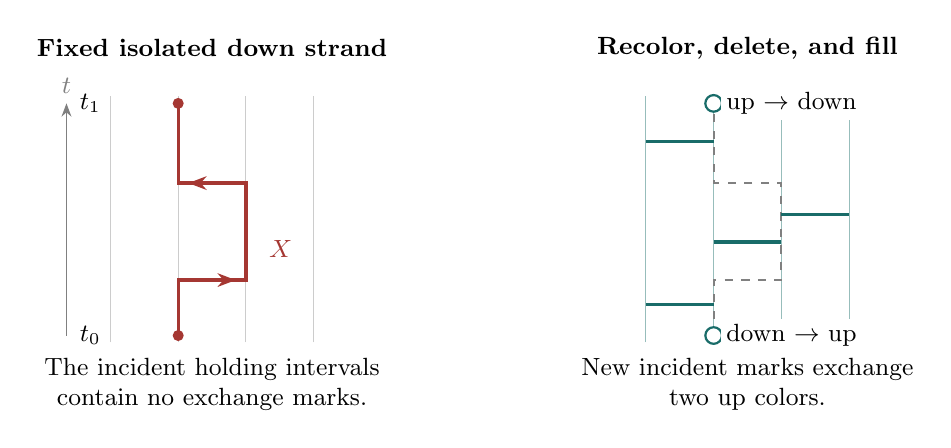
\begin{tikzpicture}[x=0.86cm,y=0.88cm,>=Stealth,
 every node/.style={font=\small}]
 \definecolor{downpath}{RGB}{165,55,50}
 \definecolor{upfill}{RGB}{25,108,105}
 \begin{scope}
  \node[font=\small\bfseries] at (1.5,4.5) {Fixed isolated down strand};
  \foreach \x in {0,1,2,3}
   \draw[gray!40] (\x,0.25)--(\x,3.8);
  \draw[->,gray] (-0.65,0.35)--(-0.65,3.7) node[above] {$t$};
  \draw[downpath,very thick] (1,0.35)--(1,1.15)--(2,1.15)--(2,2.55)--(1,2.55)--(1,3.7);
  \draw[downpath,->,thick] (1.2,1.15)--(1.85,1.15);
  \draw[downpath,->,thick] (1.8,2.55)--(1.15,2.55);
  \fill[downpath] (1,0.35) circle (2pt);
  \fill[downpath] (1,3.7) circle (2pt);
  \node[left] at (0,0.35) {$t_0$};
  \node[left] at (0,3.7) {$t_1$};
  \node[right,align=left,text=downpath] at (2.2,1.6) {$X$};
  \node[align=center] at (1.5,-0.35) {The incident holding intervals\\contain no exchange marks.};
 \end{scope}
 \begin{scope}[xshift=6.8cm]
  \node[font=\small\bfseries] at (1.5,4.5) {Recolor, delete, and fill};
  \foreach \x in {0,1,2,3}
   \draw[upfill!45] (\x,0.25)--(\x,3.8);
  \draw[gray,dashed,thick] (1,0.35)--(1,1.15)--(2,1.15)--(2,2.55)--(1,2.55)--(1,3.7);
  \foreach \x/\y in {0/0.8,1/1.7,2/2.1,0/3.15}
   \draw[upfill,very thick] (\x,\y)--++(1,0);
  \draw[upfill,fill=white,thick] (1,0.35) circle (3pt);
  \draw[upfill,fill=white,thick] (1,3.7) circle (3pt);
  \node[right,fill=white,inner sep=2pt] at (1.1,0.35) {down $\to$ up};
  \node[right,fill=white,inner sep=2pt] at (1.1,3.7) {up $\to$ down};
  \node[align=center] at (1.5,-0.35) {New incident marks exchange\\two up colors.};
 \end{scope}
\end{tikzpicture}
\caption{The color-counting comparison for a fixed isolated strand.
Time runs upwards; horizontal segments represent instantaneous exchanges,
and the slot coordinates are schematic. Recoloring the prescribed segment
$X$ up allows its jump marks to be removed and its incident holding intervals
to be filled freely. The only remaining color discontinuities are the two
directed endpoint flips. Each cycle meeting a flip has at most one admissible
coloring, which gives the pin-weight bound used in the path comparison.}
\label{fig:surgery}
\end{figure}


In particular, \eqref{eq:isolateddomination} bounds a joint event, not
the strand law conditioned on isolation.  This is precisely what is
needed when excluding rare isolated strands with large displacement.

\begin{proposition}[Good exposures]\label{prop:good}
Under $\PP_P$ there is an event $\mathcal G$ with
\begin{equation}\label{eq:goodprob}
 \PP_P(\mathcal G^c)=o(\beta^{-5/2})
\end{equation}
having the following properties in $B_{12R_*}(x)$, in either direction
of traversal.
\begin{enumerate}
\item A strand makes at most $c_0L$ inter-site steps in a block and at
most $C\log\beta$ in a bin.  The bounds also apply to segments traced
from an intermediate visit to the region, in either time direction.
\item At each block cut, every ball of radius $c_1L$ centered in the
region contains at most five obstacle slots.  Local regularity at
radius $R_*$ about $x$ holds at all times.  In every block, the set of
fully regular times at that radius has length at least half the block.
\item A strand is called isolated in a block and direction if no other
obstacle slot lies within $c_2L$ of its starting site.  Every such
strand stays at distance greater than two from all other obstacles
and has maximal site displacement at most $CL^{3/4}$ in the block.
\end{enumerate}
The constants are fixed in the order $c_0$, then $c_2$, then $c_1$,
with each sufficiently large for the preceding choices.  The event
and all its properties repeat on subsequent copies of the period.
\end{proposition}

\begin{proof}
First control the number of strand steps.  A chronological connected
list of $j$ inter-site marks in an interval of length $u$, anchored at
a prescribed site, has probability at most
\begin{equation}\label{eq:marklist}
 \frac{(Cu)^j}{j!}.
\end{equation}
Indeed, there are at most $C^j$ successive site and slot-edge choices,
and the ordered time simplex has volume $u^j/j!$; apply the factorial
bound in Proposition~\ref{prop:loopinputs}.  The same count works in
reverse order.  It bounds lists anywhere in the interval, so it also
covers a segment beginning at an arbitrary intermediate visit; no
union over real starting times is necessary.  Taking $j=c_0L$ on
blocks, with $c_0$ large, gives $e^{-cL}$ tails.  Taking
$j=C\log\beta$ on bins gives rapidly small tails by the factorial in
\eqref{eq:marklist}.  A polynomial union over sites, blocks, bins, and
both directions proves the first property with rapidly small error.
For this count and the next one enlarge the region to $B_{20R_*}(x)$.

At a fixed block cut and center, six obstacles in a ball of radius
$c_1L$ supply six distinct slot points there.  There are at most
$CL^{18}$ such six-tuples.  Proposition~\ref{prop:snapshot}, followed
by a union over centers and at most $C\beta$ cuts, bounds this failure
probability by
\begin{equation}\label{eq:sixfailure}
 C\beta R_*^3L^{18}\lambda^6
       \le C\beta^{-3+18\delta}
       =C\beta^{-2.91}=o(\beta^{-5/2}).
\end{equation}
Seam permutations preserve the site counts, including multiplicities,
so this estimate holds on either seam side.

If six blocked sites were present in one of the required fixed-radius
balls during a block, one obstacle at each site could be traced back
to the block cut.  The first property would place their six distinct
starting slots in a ball of radius $c_1L$, once $c_1$ is large enough.
This is impossible.  Thus local regularity holds at all times.
For the remaining condition, Proposition~\ref{prop:geometryinputs}
bounds the expected measure of times when distant-component regularity
fails in any block $I$ by $C|I|e^{-cR_*^\xi}$.  Markov's inequality
and a union over blocks show, with rapidly small error, that it fails
on less than half of every block.  This proves the second property.

The step bound also ensures that an isolated strand cannot meet another
obstacle during its block.  Any potential encounter can be traced back
in both strands to their distinct block-start slots, at total distance
at most a fixed multiple of $c_0L$.  Choose $c_2$ larger than that
multiple.  This argument also covers strands entering the region,
by tracing backward from the encounter.

It remains to bound the isolated strand's displacement.  The site
coordinate of the base walk in Lemma~\ref{lem:isolatedpath} jumps at
rate $S$ to each nearest neighbor.  Exponential martingales in each
coordinate give, for $u\le2L$,
\[
 \PP_{\mathrm b}\left(\max_{0\le v\le u}
                   |X(v)-X(0)|_\infty>CL^{3/4}\right)
       \le C e^{-c\sqrt L}.
\]
For example, use an exponential parameter of order $L^{-1/4}$; the
martingale compensator is at most a constant times $uL^{-1/2}$.
On the step event already established, strands beginning in the
region stay interior.  Lemma~\ref{lem:isolatedpath} therefore bounds
the joint event of isolation and excessive displacement.  A polynomial
union over slots, blocks, and directions is rapidly small.  Seams make
no spatial displacement; for a seam block, enumerate also the slots
on its other seam side.  Combining these exceptional sets proves
\eqref{eq:goodprob} and the third property.
\end{proof}

\subsection{Heat propagation at a fixed good exposure}

From this point, all actual kernels kill on $E$, not at $i$.
The estimates in this subsection are deterministic statements about
the fresh walk at an exposure in $\mathcal G$.  The earlier picture
probabilities have already done their work in constructing that event.

\begin{lemma}[Local heat bound]\label{lem:heatbound}
On $\mathcal G$, a fresh-walk interval kernel of elapsed length $u$,
additionally killed on exit from $B_{R_*}(x)$, has maximum entry at most
\begin{equation}\label{eq:heatbound}
 C(1+u)^{-3/2}.
\end{equation}
The bound holds for either time direction, for every starting slice,
with additional spatial killing, and across copies of the period.
\end{lemma}

\begin{proof}
We use Nash's energy-dissipation argument
\cite[pp.~935--936]{Nash1958}.
For a nonnegative input of mass at most one, let $l=\norm{v}_2^2$.
The all-time local regularity in Proposition~\ref{prop:good} permits
\eqref{eq:nash} at every smooth time, so
$l'\le-cl^{5/3}$.  Instantaneous operations are contractions by
Lemma~\ref{lem:kernelenergy}.  Integrating gives
$\norm{v}_2\le C(1+u)^{-3/4}$ for a unit point input.
Split the kernel at its midpoint and express an entry as the inner
product of a forward mass and an adjoint mass, each propagated for
$u/2$.  Their two norm bounds give \eqref{eq:heatbound}.
\end{proof}

\begin{lemma}[Displacement of the fresh walk]\label{lem:localization}
On $\mathcal G$, from any slot above $B_{6R}(x)$ and any starting
slice, a fresh walk run for elapsed time $u\le2\beta$ in either
direction stays within site distance
\begin{equation}\label{eq:localization}
 C(1+u/L)L^{3/4}
\end{equation}
of its starting site, apart from a rapidly small probability uniform
over the fixed good exposure.  The assertion bounds the probability
of excessive displacement before killing.  In particular, adding
killing on exit from $B_{R_*}(x)$ changes these propagations by a
rapidly small amount in total mass.
\end{lemma}

\begin{proof}
Consider first a piece of one block, of length at most $2L$, starting
at any slice and over a site $z$ in $B_{9R}(x)$.  Stop on exiting
$B_L(z)$, including its exit step in the displacement estimate.
Every obstacle strand visiting this ball or its immediate neighbors
traces back at most $c_0L$ steps to a distinct slot at the deterministic
block cut.  The obstacle count in Proposition~\ref{prop:good} thus
shows that at most five strands can be relevant before stopping.
Their instantaneous neighborhoods have uniformly bounded size.

The rate jumps of each site coordinate have bounded rates and unit
increments.  Their drift vanishes away from the neighboring obstacles
and is uniformly bounded elsewhere.  Lemma~\ref{lem:heatbound}, with
the stopping-ball killing, bounds the expected occupation time near
the relevant strands by
\[
 C\int_0^{2L}(1+t)^{-3/2}\,dt\le C.
\]
The expectation is uniform in the starting slot and slice, including
either side of any prescribed operation.

A forced transport occurs only when the fresh walk is at its prescribed
departure hole.  In any bin there are at most $C\log\beta$ relevant
transports, by the bin step bound for the five strands.  Apply
\eqref{eq:heatbound} to the probability of presence just before each
such operation.  Summing over bins, using their lengths between one
and three, bounds the expected number of forced steps before stopping
by
\[
 C\log\beta\sum_{n\ge0}(1+n)^{-3/2}\le C\log\beta.
\]
The same estimate holds from an arbitrary intermediate slice: a
unit-time interval intersects only a bounded number of the original
bins.  These estimates use deterministic transport times at fixed
exposure, with no conditional Poisson assertion.

Let $A$ be the accumulated occupation time near obstacles plus the
number of forced steps.  From every stopping slice and surviving
state, the conditional expected remaining accumulation is at most
$C\log\beta$.  The Markov property and Markov's inequality show
that each further increment of size $2C\log\beta+1$ has conditional
probability at most $1/2$.  Occupation time is continuous and the
transport-count overshoot is at most one.  Restarting at successive
thresholds therefore gives, for each fixed $a>0$,
\[
 \Pr(A>aL^{3/4})\le C_a
        \exp\{-c_aL^{3/4}/\log\beta\}.
\]
This controls both the integrated drift and the forced displacement.

Subtract the integrated drift from the ordinary rate jumps.  For each
coordinate, bounded rates and unit jumps imply that its compensated
process $M_t$ has
$\exp\{\theta M_t-C\theta^2t\}$ as a supermartingale for
$|\theta|\le1$, with a fixed $C$.  The maximal inequality with
$\theta$ of order $L^{-1/4}$ gives
\[
 \Pr\bigl(\max_{t\le2L}|M_t|>aL^{3/4}\bigr)
                                  \le C_a e^{-c_a\sqrt L}.
\]
The three displacement contributions prove the claimed bound on one
block piece.  Since $CL^{3/4}<L$ for large $\beta$, they also bound
the probability of reaching the stopping sphere.  Seam operations
change no site coordinate.

An interval of length $u$ meets at most $C(1+u/L)$ block pieces.
Apply the preceding uniform bound successively and add their
displacements.  There are polynomially many pieces, so the total
failure probability remains rapidly small.  Throughout an interval
of length at most $2\beta$, the resulting displacement is
$O(\beta L^{-1/4})=o(R)$.  The walk therefore stays in the local
region used above, and in $B_{R_*}(x)$.  This proves the lemma.
\end{proof}

\subsection{Overlaps of flows}

The final geometric estimate measures the energy cost of superposing
flows from different source locations.  It retains their separation,
which will be essential when averaging the sparse source locations.

\begin{lemma}[Flow overlap]\label{lem:flowoverlap}
At a fully regular slice on $\mathcal G$, choose the unit flows in
\eqref{eq:flowenvelopes} for available slots $a,a'$ over $B_{6R}(x)$.
Then
\begin{equation}\label{eq:flowoverlap}
 \sum_e|J_a(e)J_{a'}(e)|
       \le\frac{C}{1+\dist(a,a')},
\end{equation}
where the distance is between their sites.
\end{lemma}

\begin{proof}
Where both edge distances from the source sites are at most $R_*$,
use the two inverse-square envelopes.  Their convolution in dimension
three is bounded by $C/(1+b)$ at source separation $b$: balls of
radius $b/2$ about either source contribute $C/(1+b)$, and dyadic
shells outside them have the same total bound.

If one source distance exceeds $R_*$, both are at least a fixed
multiple of $R_*$, since $a,a'$ lie over $B_{6R}(x)$ and $R=o(R_*)$.
The global envelopes then bound the remaining sum by
\[
 C R_*^{3-2(199/100)}
       =C R_*^{-98/100}
       \le C R^{-1}.
\]
The last inequality follows from
$(5/3)(98/100)=49/30>3/2+\delta/4$.
As $b\le12R$, this is bounded by the right-hand side of
\eqref{eq:flowoverlap}.
\end{proof}

\section{The ideal potential and its profiles}\label{sec:profiles}

We now choose the trial vector for the capacity comparison.
The free potential includes every positive number of periods, so its
capacity already contains the full ideal-magnon density.  A spatial
cutoff makes it a finite-volume test vector without truncating those
periods.  We also obtain the spatial and temporal estimates needed to
compare its evolution with the walk among holes.

Fix $S$, put $\ell=2S$, and use the scales in \eqref{eq:scales}.
Let $E=D_0\cup F$, where $F$ is a finite deterministic set of
slot-time pins, and let $i=(x,a)$ be an unpinned post-seam slot at time
zero.  Throughout the comparison assume that $B_{50R_*}(x)$ lies in
the interior of the cube and that no point of $E$ lies above this
ball.  The picture law is $\PP_P$, where $P=E\cup\{i\}$.
At a fixed exposure let $U$ be the forward one-period kernel killed
on $E$, retaining its zero rows and columns on killed cut slots.
Set $A=I-U$ and use the energy $e_y$ of
Section~\ref{sec:capacity}.

\subsection{The all-turn free potential}

On $\Z^3\times\{1,\ldots,\ell\}$, let $\mathscr L$ have rate
$1/2$ on every slot edge, and let $T_s=\exp(s\mathscr L)$.
Let $J$ be the projection that averages the slots at each site.
For a slot-uniform vector the site jump rate is $\ell/2=S$ to each
neighbor.  Denote this site semigroup by $P_s$, and its kernel from
the origin by $p_s(z)$.  Its Fourier multiplier is
\begin{equation}\label{eq:freemultiplier}
 \widehat p_s(k)
 =\exp\!\left[-2sS\sum_{j=1}^3(1-\cos k_j)\right],
 \qquad k\in[-\pi,\pi]^3.
\end{equation}
If a vector has zero sum on the slots at every site, then
$\mathscr L$ acts on it as $-3\ell I$.  Therefore
\begin{equation}\label{eq:slotdecomposition}
 T_s=P_sJ+e^{-3\ell s}(I-J).
\end{equation}
The free seam is $J$.  It commutes with $T_s$, so the ideal full-period
operator, in either direction, is
\[
 U_0=JT_\beta=T_\beta J=P_\beta J,
 \qquad
 (U_0^n)_{(z,b),(x,a)}=\frac1\ell p_{n\beta}(z-x)
 \quad(n\ge1).
\]
In particular the slot modes removed by the seam contribute nothing
to a positive full turn.

With $\eta=\ind_{\{i\}}$ on the full slot lattice, define the
slot-uniform function
\begin{equation}\label{eq:freepotential}
 v(z)=\frac1\ell\sum_{n\ge1}p_{n\beta}(z-x),
 \qquad c=\frac1{1+v(x)}.
\end{equation}
The estimates below show that the sum is finite and
$v(x)=O_S(\beta^{-3/2})$.  Positivity and the semigroup property give
\begin{equation}\label{eq:freepotentialidentity}
 U_0(\eta+v)=v.
\end{equation}
Choose $\chi:\R^3\to[0,1]$ smooth, equal to one when
$|z-x|_\infty\le R/2$ and zero when $|z-x|_\infty\ge R$, with
first and second derivatives bounded by $C/R$ and $C/R^2$.
Use its restriction to sites as a slot-uniform
multiplier.  The full trial vector is
\begin{equation}\label{eq:trialvector}
 h=c\chi(\eta+v),
\end{equation}
and the same symbol denotes its restriction to the cut holes.
It vanishes on every killed cut slot and satisfies $h(i)=1$.
Moreover $p_s(z)\le p_s(0)$, by the Fourier representation, so
$0\le h\le1$.

\subsection{Forward and reverse profiles}

Put $g=c(\eta+v)$ on the full slot lattice.  The forward and reverse
profiles, before restriction to holes, are
\begin{align}
 a_s&=\chi T_s g\quad(0\le s<\beta),
 &a_\beta&=\chi JT_\beta g,                         \label{eq:forwardprofile}\\
 b_0&=\chi g,\qquad b_{0+}=\chi Jg,
 &b_s&=\chi T_sJg\quad(0<s\le\beta).                 \label{eq:reverseprofile}
\end{align}
Here $s$ is elapsed time in the indicated direction.  The forward
traversal contains the seam at its end.  The reverse traversal contains
it at its beginning, with $b_0$ its incoming value and $b_{0+}$ its
outgoing value.  Each traversal includes the seam exactly once.
At every slice, the same symbols also denote the restrictions to the
holes on the specified side of any instantaneous operation; ``full
profile values'' will always refer to the formulas before restriction.

Multiplication by $\chi$ commutes with $J$.  Thus the full profiles
undergo the ideal seam operation, and \eqref{eq:freepotentialidentity}
gives the endpoint identities
\begin{equation}\label{eq:profileendpoints}
 a_0=b_0=h,\qquad a_\beta=b_\beta=h-c\eta.
\end{equation}
The smooth part of either profile is the contribution of $cv$;
the point part is the contribution of $c\eta$.  This decomposition
also applies to full profile values.

For $r_z=|z-x|_\infty$ and $d\ge1$, introduce
\begin{equation}\label{eq:weights}
 \begin{split}
 G(z)&=\beta^{-1}(D_*+r_z)^{-1},\qquad
 W(z)=\beta^{-1}(D_*+r_z)^{-2},\\
 P_d(z)&=d^{-3}(1+r_z/d)^{-12},\qquad
 W_d(z)=d^{-4}(1+r_z/d)^{-12}.
 \end{split}
\end{equation}
For a slot function $u$, a bounded-distance difference at $z$ means
$u(z,a)-u(z',a')$ with $|z-z'|_\infty$ at most a fixed constant;
the constants below may depend on that constant.  This includes
differences between two slots at the same site.

\begin{lemma}[Bounds for the free profiles]\label{lem:freebounds}
For fixed $S$ and all sufficiently large $\beta$, the following
bounds hold uniformly in the direction, elapsed time, site, and slot.
For the full smooth profile $u_s$, its absolute value,
bounded-distance differences, and open-interval time derivative are
bounded, respectively, by
\begin{equation}\label{eq:smoothbounds}
 C G(z),\qquad C W(z),\qquad C W(z)/D_*.
\end{equation}
For the full point profile $w_s$, put $d=\sqrt{1+s}$.
The corresponding bounds are
\begin{equation}\label{eq:pointbounds}
 C P_d(z),\qquad C W_d(z),\qquad C W_d(z)/d.
\end{equation}
The smooth profile is slot-uniform and does not change at the seam.
The slot differences and seam changes of the point profile satisfy
the difference bound in \eqref{eq:pointbounds}.
For each fixed $a>0$, when $s\ge a\beta$ the bounds
\eqref{eq:smoothbounds} also hold for $w_s$, with a constant depending
on $a$.
\end{lemma}

\begin{proof}
We first record the heat-kernel estimates before applying the cutoff.
For every fixed integer $m\ge0$ and $j=0,1,2$, Fourier inversion gives
\begin{equation}\label{eq:heatderivative}
 |\nabla^j p_t(z)|
 \le C_{m,j}(1+t)^{-(3+j)/2}
       \left(1+\frac{|z|_\infty}{\sqrt{1+t}}\right)^{-m}.
\end{equation}
Here $j$ nearest-neighbor differences may be taken in arbitrary
coordinate directions.  One time derivative satisfies the same bound
with $j=2$.
To verify the estimates, write
$\omega(k)=2S\sum_j(1-\cos k_j)$ and use
$\omega(k)\ge c_S|k|^2$ on $[-\pi,\pi]^3$.
A $j$-fold difference inserts a multiplier vanishing to order $j$
at zero; a time derivative inserts $-\omega$, which vanishes to
order two.  The integral without frequency differentiation is thus
$O((1+t)^{-(3+j)/2})$.
For the spatial weight, integrate by parts $m$ times in a coordinate
for which $|z_j|=|z|_\infty$.  The integral of the absolute value
of the differentiated multiplier is at most
$C_{m,j}(1+t)^{(m-3-j)/2}$: near zero this follows by rescaling
$k$ by $(1+t)^{-1/2}$, using
$\nabla\omega=O(|k|)$ and bounded higher derivatives; away from
zero the exponential dominates every power of $t$.
The periodic integrands have no boundary terms.  Combining this
bound with the bound without integration by parts proves
\eqref{eq:heatderivative}.  The case $0\le t\le1$ follows from
uniform bounds on the same derivatives.

The slot-uniform part of the smooth evolution is a sum of site kernels
at times $n\beta+s$, $n\ge1$.  For $j=0,1,2$, choose $m>j+1$ in
\eqref{eq:heatderivative}.  Splitting the time sum at $n\beta+s$
of order $r_z^2$, or comparing it with its integral on dyadic
intervals, gives
\begin{equation}\label{eq:heatsum}
 \sum_{n\ge1}(n\beta+s)^{-(3+j)/2}
     \left(1+\frac{r_z}{\sqrt{n\beta+s}}\right)^{-m}
 \le \frac{C}{\beta}(D_*+r_z)^{-1-j}.
\end{equation}
For completeness, when $r_z\le D_*$ the sum without its spatial
factor is $O(\beta^{-(3+j)/2})$.  When $r_z>D_*$, the terms with
$n\beta+s\ge r_z^2$ sum to $C\beta^{-1}r_z^{-1-j}$.
For the remaining terms, use the bound
$(1+r_z/\sqrt t)^{-m}\le(\sqrt t/r_z)^m$ and sum
$t^{(m-3-j)/2}$ up to $r_z^2$; the same bound results.
This proves \eqref{eq:heatsum} and the asserted pointwise convergence
of $v$.
It gives the value and difference estimates in
\eqref{eq:smoothbounds}; for time derivatives use
\[
 \beta^{-1}(D_*+r_z)^{-3}\le W(z)/D_*.
\]

For the point part, \eqref{eq:heatderivative} gives
\eqref{eq:pointbounds} with $m=12$.  Formula
\eqref{eq:slotdecomposition} adds only a site-supported slot deviation
decaying as $e^{-3\ell s}$.  This deviation, its spatial differences,
and its time derivative satisfy the same bounds, with constants
depending on $S$.  In the reverse direction the initial seam removes
that deviation; at a seam its change is bounded by the incoming
absolute value of the slot deviation and hence by $C W_d(z)$.
The smooth part is unchanged
because it is slot-uniform.

It remains to justify multiplication by $\chi$.  Value and time
derivative estimates are preserved.  In a spatial difference the
extra term contains a difference of $\chi$, supported where
$r_z$ is of order $R$.  There
$G(z)/R\le C W(z)$, and
$P_d(z)/R\le C W_d(z)$ since $d\le\sqrt{1+\beta}\ll R$.
Thus the difference estimates are preserved as well.
Finally, if $s\ge a\beta$, then $d$ is comparable with $D_*$;
direct comparison of the envelopes gives
$P_d\le C_aG$, $W_d\le C_aW$, and
$W_d/d\le C_aW/D_*$.  This proves the last assertion.
\end{proof}

At the source site, the free potential therefore recovers the ideal
density exactly.  Fourier inversion and monotone convergence give
\begin{equation}\label{eq:freeidealdensity}
 \begin{split}
 \ell v(x)=\sum_{n\ge1}p_{n\beta}(0)
 &=\int_{[-\pi,\pi]^3}\frac{d^3k}{(2\pi)^3}
      \sum_{n\ge1}e^{-2n\beta S\sum_j(1-\cos k_j)}\\
 &=n_S^{\rm sw}(\beta).
 \end{split}
\end{equation}
The integral is finite in dimension three, also as a consequence of
the heat-kernel sum in \eqref{eq:heatsum}.

The uncut potential need not be square summable.  Its evolutions
above are defined pointwise by the convergent positive series, while
the trial vector and every restricted profile used in a finite cube
have finite support.
Equation~\eqref{eq:freeidealdensity} identifies $v(x)$ with the
target in Proposition~\ref{prop:comparison}.  It remains to bound
the change of return capacity when the ideal period is replaced by
the walk among holes.
Define $\mu_+,\mu_-$ from this $h$ and $c$ by
\eqref{eq:capacityresiduals}.  Section~\ref{sec:sources} realizes
these residuals as propagated local errors of the profiles.

\section{Comparison sources and their cancellation}\label{sec:sources}

We now express the errors of the trial potential as sources in the
actual heat equation.  The key fact is a conservation identity: along
an isolated obstacle, the signed source is an endpoint difference of
the profile, up to its cutoff commutator.  Its size is therefore controlled by the obstacle's
displacement, although the total variation of the source counts every
jump.  We establish this identity before using it to estimate either
the scalar or the energy pairing.

Throughout this section we impose the interiority and absence of pins
over $B_{50R_*}(x)$ required in Section~\ref{sec:profiles}.  Constants
are uniform in the finite cube, the allowed pin set, and the injection
slot.  The two traversals and their profiles are those defined there:
$a_s$ is the forward profile and $b_s$ is the reverse profile, each
indexed by its own elapsed time $s\in[0,\beta]$.  Profiles are evaluated
on the full slot lattice before restriction to the current holes.

\subsection{Sources on intervals and at operations}

Fix one of the two directions and write $\varphi_s$ for its profile.
On an open interval containing no instantaneous operation, let
$\mathscr L_s^{\mathrm{act}}$ be the generator on the holes, with the
prescribed killing.  The continuous source is the vector
\begin{equation}\label{eq:continuous-source}
 \mathscr L_s^{\mathrm{act}}(\varphi_s|_{H_s})
             -(\partial_s\varphi_s)|_{H_s}.
\end{equation}
Here $H_s$ denotes the hole set on the slice.  At an instantaneous
transition $K:\R^{H_-}\to\R^{H_+}$, the atomic source, on the outgoing slice, is
\begin{equation}\label{eq:atomic-source}
 K(\varphi_-|_{H_-})-\varphi_+|_{H_+}.
\end{equation}
In reverse time these are the transposed maps, in reverse order.
Thus a reverse atomic source lies before the
operation when viewed in forward time.

Write $s^+$ and $s^-$ for these collections of continuous densities
and atomic vectors in the forward and reverse traversals.  Integrating
against a collection will mean a Lebesgue integral of its continuous
part plus the sum over its atoms.  Every source is supported above
$B_{R+2}(x)$.  There are no pins of $E$ or boundary slots in this region,
so killing creates no additional source there.

There are two types of source.  The first is the cutoff commutator,
defined on the full lattice by
\begin{equation}\label{eq:backgroundsource}
 \gamma_s=\mathscr L\varphi_s-\partial_s\varphi_s,
 \qquad b_*:=\beta^{-1}R^{-3}.
\end{equation}
The uncut profile solves the free heat equation.  Consequently
$\gamma_s$ is supported where $R/3\le r_z\le2R$, and
\begin{equation}\label{eq:backgroundbound}
 |\gamma_s(z,a)|\le Cb_*.
\end{equation}
These assertions hold separately for the smooth part and the point
part of either profile.  Indeed the commutator of $\mathscr L$ with
$\chi$ consists of a cutoff second difference times a profile value,
and products of first differences.  On this annulus,
Lemma~\ref{lem:freebounds} gives values at most $C/(\beta R)$ and
first differences at most $C/(\beta R^2)$, uniformly in elapsed time.
The bounds on the cutoff derivatives prove
\eqref{eq:backgroundbound}.  There is no cutoff atom at the seam,
because the sitewise cutoff commutes with both full-profile seam
averaging and restriction within a site.

The remaining sources come from obstacles.  A removed edge from a
hole $j$ to an obstacle $k$ contributes
\begin{equation}\label{eq:removed-edge-source}
 \tfrac12(\varphi_s(j)-\varphi_s(k))
 \quad\text{at the hole }j.
\end{equation}
If an obstacle moves from $k$ to a hole $j$, the hole moves from $j$
to $k$.  The source on this arriving hole is
\begin{equation}\label{eq:transport-source}
 \varphi_s(j)-\varphi_s(k).
\end{equation}
Exchanges between two obstacles create no source.  At a seam the
source is the difference between the actual average on the remaining
hole slots and the full-profile average, restricted to the outgoing
holes.  It vanishes at sites with no obstacles.

Assign a removed-edge source to its obstacle and a transport source
to the obstacle responsible for the transport.  Assign seam sources
at a site to its obstacle strands, in any fixed manner.  If a strand
is isolated, it is the only obstacle there and receives the entire
seam source at that site.  These assignments can be made either in
a block or in a bin, with strands enumerated at its initial slice
in the direction being used.
On $\mathcal G$, tracing a strand back from a source site in
$B_{R+2}(x)$ uses at most $CL$ steps in its block, by
Proposition~\ref{prop:good}.  Thus every strand contributing a
nonzero source starts in $B_{4R}(x)$, for large $\beta$.
All subsequent strand sums are restricted to this ball.

\subsection{Conservation along an isolated strand}

\begin{lemma}[Signed source identity]\label{lem:signedsource}
Fix a good picture in $\mathcal G$ and one directed block $I=[u,v]$.
Let $Z_s$ be an isolated obstacle strand starting above $B_{4R}(x)$
on this block, with its specified sides at operations.  For either
profile part, the total signed mass of the assigned obstacle sources,
obtained by summing over source slots and integrating in time, is
\begin{equation}\label{eq:signedsource}
 \varphi_v(Z_v)-\varphi_u(Z_u)
                  +\int_u^v\gamma_s(Z_s)\,ds.
\end{equation}
The endpoint values include any seam assigned to the block.  The same
formula holds in reverse elapsed time.
\end{lemma}

\begin{proof}
At every smooth time, all neighboring slots of $Z_s$ are holes, by
isolation.  Summing \eqref{eq:removed-edge-source} over these slots
therefore gives
\[
 \frac12\sum_{j\sim Z_s}
             (\varphi_s(j)-\varphi_s(Z_s))
 = (\mathscr L\varphi_s)(Z_s)
 = (\partial_s\varphi_s)(Z_s)+\gamma_s(Z_s).
\]
The transport contribution \eqref{eq:transport-source} is exactly
the profile increment along each jump of $Z_s$.

It remains to check the seam, where the two hole sets can differ.
At the strand's site let $H_-,H_+$ be the incoming and outgoing holes,
and let $Z_-,Z_+$ be the corresponding obstacle slots.  The actual
hole map preserves the sum over holes.  The full-profile seam
preserves the sum over all slots.  Since the obstacle is the only
one at this site, the total seam source is exactly
\begin{align*}
 \sum_{H_+}(K\varphi_- -\varphi_+)
 &=\sum_{H_-}\varphi_- -\sum_{H_+}\varphi_+\\
 &=\varphi_+(Z_+)-\varphi_-(Z_-).
\end{align*}
Thus it also supplies the increment along the obstacle strand.
Integrating the time derivatives and summing all increments
telescopes to \eqref{eq:signedsource}.  Reverse traversal has the
same conservation of counting sums and uses the inverse transport,
so this proof applies with reverse elapsed time as well.
\end{proof}

We next turn this identity into bounds that retain both the signed
mass and the total variation.  Keeping the two quantities separate
is essential: total variation controls propagation and localization,
whereas the smaller signed mass controls long spatial scales.

\begin{lemma}[Block source bounds]\label{lem:cancellation}
On a picture in $\mathcal G$, let a strand start above
$z\in B_{4R}(x)$ in a directed block of length between $L$ and $2L$.
For the smooth profile part, take $\mathcal W=W$.
For a point-profile part, suppose that $d=\sqrt{1+s}$ is comparable
throughout the block and $\inf d\ge L$, and take $\mathcal W=W_d$
at its starting elapsed time.  Then the obstacle sources assigned
to this strand are supported within distance $CL$ of $z$ and have
total variation at most
\begin{equation}\label{eq:blocksourcevariation}
 CL\mathcal W(z).
\end{equation}
If the strand is isolated, their signed sum has absolute value at most
\begin{equation}\label{eq:blocksourcecancellation}
 CL^{3/4}\mathcal W(z).
\end{equation}
Both assertions also hold with $\mathcal W=W$ for the point profile
on blocks in the second half of elapsed time, and for the sum of that
part and the smooth part, after changing the constant.
\end{lemma}

\begin{proof}
The step bounds in Proposition~\ref{prop:good} keep the strand and
its adjacent source sites within $CL$ of its starting site.  The
weights $W$ are comparable throughout this region, because $L\ll D_*$.
The stated hypotheses give the same comparability for $W_d$.
Each strand has bounded degree, contributes for at most $2L$ units
of continuous time, and makes at most $CL$ jumps.  The difference
bounds of Lemma~\ref{lem:freebounds}, together with
\eqref{eq:removed-edge-source} and \eqref{eq:transport-source},
give \eqref{eq:blocksourcevariation}.  At a seam, fixed slot
multiplicity bounds the number of terms, and the difference of the
two averages is bounded by the slot-difference bound.  This adds at
most $C\mathcal W(z)$.

For an isolated strand use Lemma~\ref{lem:signedsource}.  Its endpoint
displacement is at most $CL^{3/4}$.  The spatial endpoint difference
therefore costs at most $CL^{3/4}W(z)$ in the smooth case.  Time
variation costs $CLW(z)/D_*$, and a seam increment costs at most
$CW(z)$.  On the cutoff annulus,
$b_*\le CW(z)/D_*$, so the integral in
\eqref{eq:signedsource} has the same time bound.  Since
$1+L/D_*\le CL^{3/4}$, this proves
\eqref{eq:blocksourcecancellation} for the smooth part.

For the point part the time derivative is bounded by $CW_d/d$.
On the cutoff annulus its commutator is bounded by
\[
 C\bigl(W_d/R+P_d/R^2\bigr)\le CW_d/d,
\]
because $d\le\sqrt{1+\beta}\ll R$.  The same endpoint argument
gives $C[L^{3/4}+1+L/d]W_d(z)$, which proves the stated bound.
Finally Lemma~\ref{lem:freebounds} bounds the point part by the
smooth envelopes when $s\ge\beta/2$.  Addition proves the last
assertion; the division at $\beta/2$ is a block endpoint.
\end{proof}

Near elapsed time zero, $W_d$ varies too quickly to use block
cancellation.  The bins of length between $1$ and $3$ provide the
following uniform replacement.  We write
$H_\beta=C(1+\log\beta)^C$ for a fixed power of a logarithm;
the constants, and hence this power, may be enlarged at subsequent
uses.

\begin{lemma}[Bin source bounds]\label{lem:sourcebins}
On a picture in $\mathcal G$, the obstacle sources assigned to one
strand in one directed bin, starting above $z\in B_{4R}(x)$ at elapsed time $s$,
have total variation at most
\begin{equation}\label{eq:binsourcevariation}
 H_\beta\bigl(W(z)+W_d(z)\bigr),\qquad d=\sqrt{1+s}.
\end{equation}
The two profile parts separately satisfy this bound with their own
weight.  Their source sites lie within $C\log\beta$ of $z$.
\end{lemma}

\begin{proof}
Proposition~\ref{prop:good} bounds both displacement and the number
of jumps in a bin by $C\log\beta$.  Continuous contributions have
bounded time length.  Within a bin, $1+s$ changes by a bounded
factor, while a spatial shift of $C\log\beta$ changes any of the
polynomial envelopes in Lemma~\ref{lem:freebounds} by at most a
fixed power of $1+\log\beta$.  The formulas for removed edges,
transports, and seam averaging now give the result.
\end{proof}

There are at most $CR^3$ possible starting slots in each bin and
$C\beta$ bins, while $W+W_d\le C$.  Including the background,
the total variation of either complete source collection on
$\mathcal G$ is therefore at most $CH_\beta\beta R^3$.
In particular, multiplying a rapidly small propagation error by
one or two such total variations still gives a rapidly small error.

\subsection{Propagation and the two-source identity}

Let $T_{v,u}$ denote actual forward propagation between specified
slices, including exactly the operations lying between them.
Reverse propagation is the adjoint with the ordered endpoints.
Propagate every source from its insertion slice to its terminal cut
in its own direction.  The resulting signed masses are precisely
the residuals defined in Section~\ref{sec:capacity}:
\begin{equation}\label{eq:residualdefinition}
 \mu_+=\int T_{\beta,s}\,s^+(ds)=Uh-h+c\eta,
 \qquad
 \mu_- =\int T^{\mathrm{rev}}_{\beta,s}\,s^-(ds)
                         =U^*h-h+c\eta.
\end{equation}
For example, on a smooth interval the difference between the actual
mass and the profile satisfies the actual heat equation with forcing
\eqref{eq:continuous-source}.  At an operation it is multiplied by
the actual map and then receives \eqref{eq:atomic-source}.
Telescoping from the initial profile $h$ to the terminal profile
$h-c\eta$ proves \eqref{eq:residualdefinition}.

For a scalar pairing it is useful to make this substitution twice.
Read the reverse profile at forward physical time $t$ by writing
$\bar b_t=b_{\beta-t}$, always on the specified side of an operation.
In particular it is evaluated on the outgoing slice when paired
with a forward source.

\begin{lemma}[Two-source Duhamel identity]\label{lem:duhamel}
For the comparison sources just defined,
\begin{equation}\label{eq:doubledduhamel}
 \ip{\mu_+}{h}
 =\int\ip{s^+(ds)}{\bar b_s}
  +\iint_{s\prec t}
          \ip{T_{t,s}s^+(ds)}{s^-(dt)}.
\end{equation}
In the second integral the reverse sources are indexed by forward
physical time.  The order $s\prec t$ means that the forward insertion
slice lies before the reverse insertion slice.  Thus $T_{t,s}$ runs
from after the first operation to before the later operation when
both sources are atomic.  There is no term pairing the forward and
reverse sources of the same operation.
\end{lemma}

\begin{proof}
Here is the exact telescoping calculation for instantaneous factors;
it also fixes the endpoint convention in the integrals.  Let
$K_j:V_{j-1}\to V_j$, $1\le j\le n$, be the chronological factors
between counting spaces, and write $a_j,b_j$ for comparison values
at those slices, with $a_0=b_n=h$.  In this calculation $b_j$
is indexed in forward order.  Put
\[
 p_j=K_j a_{j-1}-a_j,\qquad
 q_j=K_j^*b_j-b_{j-1},\qquad
 P_{r,l}=K_r\cdots K_{l+1}.
\]
The forward error is $\sum_jP_{n,j}p_j$.  Reverse telescoping gives
\[
 P_{n,j}^*h=b_j+\sum_{k>j}P_{k-1,j}^*q_k.
\]
Their pairing is consequently
\[
 \sum_j\ip{p_j}{b_j}
       +\sum_{j<k}\ip{P_{k-1,j}p_j}{q_k}.
\]
The indices $j<k$ express that $p_j$ is inserted after its factor,
whereas $q_j$ is inserted before that factor.  On each intervening
smooth interval the variation-of-constants formula gives the same
identity with time integrals.  Composing these formulas with the
finite telescoping calculation proves \eqref{eq:doubledduhamel}.
Two continuous source measures have no diagonal mass; atomic terms
retain the strict slice order above.  In particular the forward
terminal seam source pairs directly with $h$ in the first sum.
The reverse seam source lies before that operation and pairs only
with earlier forward sources, through kernels ending before the
seam.  No kernel in this pairing crosses that seam twice.
\end{proof}

\section{The scalar error at the trial potential}\label{sec:scalar}

The first error in the capacity comparison is the pairing of the
propagated source with the trial potential itself.  We estimate it
using Lemma~\ref{lem:duhamel}.  Its first term benefits from signed
cancellation on isolated strands.  Its second term contains two
sources, and heat-kernel decay and spatial localization make their
joint contribution smaller.  All expectations below use the actual
pin law $\PP_P$.

\begin{proposition}[Scalar estimate]\label{prop:scalar}
With the scales of \eqref{eq:scales}, under the interiority and pin
assumptions of Section~\ref{sec:profiles},
\begin{equation}\label{eq:scalarclaim}
 \EE_P\bigl[\ind_{\mathcal G}|\ip{\mu_+}{h}|\bigr]
                         =o(\beta^{-5/2}).
\end{equation}
The error is uniform in the finite cube, the deterministic pin set,
and the injection slot.
\end{proposition}

\subsection{A single source paired with the free profile}

For forward time $s$ put
\[
 d=\sqrt{1+s},\qquad d'=\sqrt{1+\beta-s}.
\]
The reverse profile $\bar b_s$ has value bound $C(G+P_{d'})$.
The basic weight integral is
\begin{equation}\label{eq:scalarweightintegral}
 \int_0^\beta\sum_{r_z\le4R}
       (W+W_d)(z)(G+P_{d'})(z)\,ds
                  \le C\beta^{-1}(1+\log\beta).
\end{equation}
To verify it, first sum the smooth product by radial shells:
\[
 \sum_{r_z\le4R}W(z)G(z)
 \le C\beta^{-2}
       \left(1+\int_0^{4R}\frac{r^2\,dr}{(D_*+r)^3}\right)
 \le C\beta^{-2}(1+\log\beta).
\]
For $s\le\beta/2$, Lemma~\ref{lem:freebounds} gives $P_{d'}\le CG$,
and
\[
 \sum_z W_d(z)G(z)
 \le \sup G\sum_z W_d(z)\le C\beta^{-3/2}d^{-1}.
\]
Integration over this half-period costs at most $C\beta^{-1}$.
For $s\ge\beta/2$, use $W_d\le CW$ and
$\sum_zP_{d'}(z)\le C$, so the remaining product costs at most
$C\sup W=C\beta^{-2}$ per unit time.  This proves
\eqref{eq:scalarweightintegral}.

Consider first the blocks contained in
$[\beta^{1/4},\beta-\beta^{1/4}]$.  On each such block
$d,d'\ge\beta^{1/8}$ and their weights are comparable over the block
and over distances $CL$.  At a deterministic initial slice,
Proposition~\ref{prop:snapshot} bounds the probability of an obstacle
at a prescribed slot by $C\lambda$.  If it is not isolated, a second
distinct obstacle lies within $c_2L$, whence the same proposition and
a union bound give
\begin{equation}\label{eq:nonisolatedprobability}
 \PP_P(\text{the prescribed slot is an obstacle and is not isolated})
                       \le CL^3\lambda^2.
\end{equation}
Here and below fixed slot multiplicities are included in constants.

For a nonisolated strand starting over $z$, the total variation
bound in Lemma~\ref{lem:cancellation} bounds its scalar contribution
by
\[
 CL(W+W_d)(z)(G+P_{d'})(z).
\]
For an isolated strand subtract from the testing profile $\bar b$
its value at the strand's initial site and time, at any one slot.
The constant value pairs with the signed source, whose bound is
$CL^{3/4}(W+W_d)(z)$.  The remaining variation of the testing profile
is at most
\begin{equation}\label{eq:profilevariation}
 CL(W+W_{d'})(z)
 \le C L\beta^{-1/8}(G+P_{d'})(z).
\end{equation}
Spatial variation follows from the difference bounds over distance
$CL$; time variation over the block follows from the time derivative
bounds.  The last inequality uses $W\le G/D_*$ and
$W_{d'}=P_{d'}/d'$.

Take expectations, use \eqref{eq:nonisolatedprobability}, and sum the
blocks.  Their lengths are comparable to $L$, so their weight sums
are bounded by $L^{-1}$ times
\eqref{eq:scalarweightintegral}.  The contribution of all these
blocks is at most
\begin{equation}\label{eq:centralfirstterm}
 C\beta^{-1}(1+\log\beta)
   \left[L^3\lambda^2
          +\lambda\bigl(L^{-1/4}+L\beta^{-1/8}\bigr)\right]
                         =o(\beta^{-5/2}).
\end{equation}
The three powers of $\beta$ are respectively
$-4+3\delta$, $-5/2-\delta/4$, and $-21/8+\delta$.
The middle term is the one for which signed cancellation is needed.

The remaining blocks lie within $2\beta^{1/4}$ of an endpoint, for
large $\beta$, because $L\ll\beta^{1/4}$.  Use the bin total
variation bound from Lemma~\ref{lem:sourcebins}, without cancellation.
Weights at times and sites within a bin change by at most $H_\beta$,
so the expected contribution is bounded by $H_\beta\lambda$ times
the integral in \eqref{eq:scalarweightintegral} restricted to these
endpoint intervals.  On the first interval the preceding estimates
give
\[
 C\left[\beta^{1/4}\beta^{-2}(1+\log\beta)
       +\beta^{-3/2}\int_0^{2\beta^{1/4}}
                              (1+s)^{-1/2}\,ds\right]
 \le C\left[\beta^{-7/4}(1+\log\beta)+\beta^{-11/8}\right].
\]
The last interval costs at most
$C\beta^{-7/4}(1+\log\beta)$.  Multiplication by
$H_\beta\lambda$ gives powers at most $-23/8$ and $-13/4$,
both strictly below $-5/2$.

The cutoff background is estimated separately.  On its annulus the
reverse profile has size at most $C/(\beta R)$, so
\begin{equation}\label{eq:scalarbackground}
 \left|\int\ip{\gamma_s|_{H_s}}{\bar b_s}\,ds\right|
 \le C\beta R^3 b_*\frac1{\beta R}
 =\frac C{\beta R}=o(\beta^{-5/2}).
\end{equation}
We have therefore bounded the first term of
\eqref{eq:doubledduhamel}.  It remains to control the interaction
between its two source collections.

\subsection{Snapshot moments for spatial boxes}

The source locations at two different times are correlated.  The
following consequence of the snapshot estimate controls their
pairing without an independence assumption.

\begin{lemma}[Box moment bound]\label{lem:boxmoment}
Partition the sites into cubes $Q$ of side comparable to $F\ge1$.
At any deterministic slice let $\mathcal O$ be its obstacle slots,
and let $w$ be a nonnegative deterministic site weight of finite
support.  With slot multiplicity in the sums, set
$A_Q=\sum_{(z,a)\in\mathcal O,\ z\in Q}w(z)$.  Then
\begin{equation}\label{eq:boxmoment}
 \left(\EE_P\sum_Q A_Q^2\right)^{1/2}
 \le C\left[
  \sqrt\lambda\,\|w\|_2
  +\lambda\left\{\sum_Q
                     \left(\sum_{z\in Q}w(z)\right)^2\right\}^{1/2}
                 \right].
\end{equation}
If two such sums are taken at different deterministic slices, the
expected sum of products over pairs of anchors at distance at most
$CF$ is bounded by a constant times the product of their respective
right sides in \eqref{eq:boxmoment}.
\end{lemma}

\begin{proof}
Expand $\sum_Q A_Q^2$.  Terms using the same slot are bounded by
$C\lambda\|w\|_2^2$ by Proposition~\ref{prop:snapshot}.  Terms using
two distinct slots, including two slots at the same site, are bounded
by $C\lambda^2\sum_Q(\sum_{z\in Q}w(z))^2$.  Taking a square root
proves \eqref{eq:boxmoment}.
At a seam the same bound holds on either side: each $A_Q$ depends
only on the number of obstacle slots at each site, and these numbers
are preserved by the seam.

Distance at most $CF$ restricts the two anchors to cubes whose
indices differ by one of a bounded number of offsets.  For each
offset, Cauchy--Schwarz in the product of the picture probability
space and the cube index set gives
\[
 \EE_P\sum_Q A_Q A'_{Q+v}
 \le\left(\EE_P\sum_Q A_Q^2\right)^{1/2}
      \left(\EE_P\sum_Q (A'_Q)^2\right)^{1/2}.
\]
Sum the bounded number of offsets.  Both factors use their own
snapshot estimate, so no joint law at the two times is required.
\end{proof}

In the applications, the weights are restricted to the deterministic
anchor region $B_{4R}(x)$.  We bound their norms by the corresponding
unrestricted envelopes.  For these weights, denote the resulting bounds by
\begin{equation}\label{eq:JB}
 \begin{aligned}
 J(d)&=C\bigl(\beta^{-3/4}d^{-5/2}
                         +\beta^{-3/2}d^{-1}\bigr),
       &&w=W_d,\\
 B(F)&=C\bigl(\beta^{-2}+\beta^{-5/2}F\bigr),
       &&w=W.
 \end{aligned}
\end{equation}
To check the first line, direct shell sums give
$\|W_d\|_2\le Cd^{-5/2}$ and $\|W_d\|_1\le Cd^{-1}$;
the square root of the squared box sums is no greater than the
total weight.  For the second line,
$\|W\|_2\le C\beta^{-1}D_*^{-1/2}$.
It remains to bound the squared box sums by $C\beta^{-2}F^2$.
Use the larger envelope $C\beta^{-1}(1+r_z)^{-2}$.
The bounded number of cubes within distance $CF$ of $x$ each have
weight sum at most $CF/\beta$.  At distance comparable to $nF$,
each cube has weight at most $C\beta^{-1}F n^{-2}$ and there are
$O(n^2)$ cubes in such a shell.  Summing their squares over $n\ge1$
gives $C\beta^{-2}F^2\sum_{n\ge1}n^{-2}$, as claimed.

The time sum of $J$ over the bins of either traversal satisfies
\begin{equation}\label{eq:Jsum}
 \sum_{\mathrm{bins}}J\bigl(\sqrt{1+s_{\mathrm{bin}}}\bigr)
                           \le C\beta^{-3/4}.
\end{equation}
Indeed the bin lengths are bounded above and below, so
$\sum(1+s_{\mathrm{bin}})^{-5/4}\le C$ and
$\sum(1+s_{\mathrm{bin}})^{-1/2}\le C\sqrt\beta$.
The latter gives $C\beta^{-1}$, which is smaller than the
right side of \eqref{eq:Jsum}.

\subsection{Two sources separated in time}

First remove interactions involving cutoff background.  Counting
mass and supremum contractions of the actual kernels imply that
two background sources cost at most
\[
 C\beta^2b_*^2R^3=CR^{-3}.
\]
For one background source, integrate its time variable and use its
supremum bound.  The resulting cost is at most $C\beta b_*$ times
the total variation of the other, obstacle, source collection.
Lemmas~\ref{lem:sourcebins} and \ref{lem:boxmoment}, or simply the
one-point snapshot bound, give
\begin{equation}\label{eq:expectedsourcevariation}
 \EE_P\left[\ind_{\mathcal G}
                \int\|s^{\pm}_{\mathrm{obs}}\|_1\right]
                  \le H_\beta\lambda(R+\sqrt\beta).
\end{equation}
For the smooth weight, use
$\sum_{r_z\le4R}W(z)\le C\beta^{-1}R$ and $O(\beta)$ bins.
For the point weight use $\sum_zW_d(z)\le C/d$ and sum in time.
Thus all terms with background are $o(\beta^{-5/2})$.

We can now assume both sources are obstacle sources.  Group their
bin pairs by dyadic scales $T\in\{1,2,4,\ldots\}$, up to a constant
times $\beta$, according to $1+t-s\asymp T$.  The scale $T=1$
also includes a bounded number of neighboring and identical bins.
Equivalently one may group by bin indices; the bin length bounds
preserve comparability away from this first scale.  For a fixed bin
there are $O(T)$ partner bins at scale $T$.

First replace each intervening propagator by its version killed on
exiting $B_{R_*}(x)$.  Every source starts in $B_{R+2}(x)$, so
Lemma~\ref{lem:localization} bounds the discarded mass by a rapidly
small quantity, uniformly on $\mathcal G$.  The source supports and
total variations are bounded by fixed powers of $\beta$, by
\eqref{eq:backgroundbound} and Lemma~\ref{lem:sourcebins}; hence the
aggregate loss in the double pairing is still rapidly small.
Lemma~\ref{lem:heatbound} now bounds each entry of the killed
kernel by $CT^{-3/2}$.  The displacement assertion in
Lemma~\ref{lem:localization} further permits us, with another rapidly
small aggregate error, to retain only anchor sites at distance at most
\begin{equation}\label{eq:scalarinteractionradius}
 F=F(T):=C(1+T/L)L^{3/4}.
\end{equation}
The $C\log\beta$ shifts from the bin anchors to insertion sites
are absorbed by $L^{3/4}$.

Apply Lemma~\ref{lem:boxmoment} with boxes of side comparable to
$F(T)$.  The two bin total variations contribute only $H_\beta$
times their anchor weights.  We treat the three possible weight
products in turn.

\paragraph{Two smooth weights.}
There are $O(\beta)$ first bins and $O(T)$ partners per first bin.
Their contribution at scale $T$ is at most
\begin{equation}\label{eq:WWscale}
 H_\beta\beta T^{-1/2}B(F)^2
 \le H_\beta\left[\beta^{-3}T^{-1/2}
                        +\beta^{-4}T^{-1/2}F^2\right].
\end{equation}
Since $F^2\le C(L^{3/2}+T^2L^{-1/2})$, the dyadic sum is at most
\begin{equation}\label{eq:WWsum}
 H_\beta\left[
       \beta^{-3}+\beta^{-4}L^{3/2}
                       +\beta^{-5/2}L^{-1/2}\right]
                         =o(\beta^{-5/2}).
\end{equation}
Here $\sum_TT^{-1/2}\le C$ and
$\sum_{T\le C\beta}T^{3/2}\le C\beta^{3/2}$.
The final term explains why a displacement bound smaller than
$T$ is needed in \eqref{eq:scalarinteractionradius}.

\paragraph{One smooth and one point weight.}
Sum the point weight over its own elapsed-time bins using
\eqref{eq:Jsum}; each such bin has $O(T)$ smooth partners.
The scale-$T$ bound is
\[
 H_\beta T^{-1/2}B(F)\beta^{-3/4}.
\]
Inserting \eqref{eq:JB} and \eqref{eq:scalarinteractionradius},
and summing dyadically, gives at most
\begin{equation}\label{eq:WPsum}
 H_\beta\left[
  \beta^{-11/4}+\beta^{-13/4}L^{3/4}
                         +\beta^{-11/4}L^{-1/4}\right]
                           =o(\beta^{-5/2}).
\end{equation}
This time the growing sum is
$\sum_{T\le C\beta}T^{1/2}\le C\sqrt\beta$.
The calculation applies whichever direction supplies the point
weight, because \eqref{eq:Jsum} holds in either elapsed-time order.

\paragraph{Two point weights.}
When $t-s\le\beta/2$, their elapsed profile times satisfy
\[
 s+(\beta-t)=\beta-(t-s)\ge\beta/2.
\]
At least one is therefore at least $\beta/4$, and its point weight
is bounded by $CW$ by Lemma~\ref{lem:freebounds}.  These pairs are
already covered by \eqref{eq:WPsum}.  The remaining pairs have
separation comparable to $\beta$.  Use the entry bound
$C\beta^{-3/2}$ and the unrestricted two snapshot pairing from
Lemma~\ref{lem:boxmoment}, with a single box containing the source
support.  Summing both time variables by \eqref{eq:Jsum} costs at most
\begin{equation}\label{eq:PPsum}
 H_\beta\beta^{-3/2}
       \left(\sum_{\mathrm{bins}}J(d)\right)^2
                   \le H_\beta\beta^{-3}.
\end{equation}

This finishes the estimate of the second term in
\eqref{eq:doubledduhamel}.  To conclude, the smallest power gains
in the entire scalar calculation are $L^{-1/4}=\beta^{-\delta/4}$
in \eqref{eq:centralfirstterm}, $\beta^{-\delta/4}$ in
\eqref{eq:scalarbackground}, and $L^{-1/2}=\beta^{-\delta/2}$ in
\eqref{eq:WWsum}.  Each dominates every fixed logarithmic power
because $\delta=1/200>0$.  All other displayed terms have larger
power margins.  Taking the expected absolute value in
Lemma~\ref{lem:duhamel} proves Proposition~\ref{prop:scalar}.

\section{Residuals in the dual energy norm}\label{sec:energy}

We now bound the two residuals from Lemma~\ref{lem:duhamel} against an
arbitrary test vector, using the one-period energy of that vector.
The scalar estimate of Section~\ref{sec:scalar} is not sufficient for
this purpose: the test vector need not resemble the free potential.
Instead, we represent propagated sources as divergences of flows and
pair those flows with the gradient of the propagated test vector.
For a group of sources associated with one obstacle strand, we first
route the signed mass to a nearby slot.  Only the resulting net mass
must then be sent to infinity.  The cancellation in
Lemma~\ref{lem:cancellation} reduces this second cost.

\begin{proposition}[Dual energy estimate]\label{prop:dualenergy}
Fix \(S\), and use the scales in \eqref{eq:scales}.  Suppose that
\(B_{50R_*}(x)\) lies in the interior of the finite cube and that no
point of \(E\) lies above this ball.  Let \(\mathcal G\) be the good
event of Proposition~\ref{prop:good}, and let \(\mu_+,\mu_-\) be the
terminal residuals in \eqref{eq:residualdefinition}.
There are nonnegative measurable functions \(X_+,X_-\) of the exposure
and a deterministic rapidly small function \(\rho(\beta)\) such that,
on \(\mathcal G\),
\begin{equation}\label{eq:dualenergy}
 \abs{\ip{\mu_d}{y}}
 \le X_d\sqrt{e_y}+C_0\rho(\beta),
 \qquad d\in\{+,-\},
\end{equation}
for every real cut vector \(y\) that vanishes on the cut killing slots
and satisfies \(\norm{y}_\infty\le C_0\).  The functions \(X_d\) do not
depend on \(y\) or \(C_0\), and
\begin{equation}\label{eq:dualenergyexpectation}
 \EE_P\!\left[\ind_{\mathcal G}(X_+^2+X_-^2)\right]
 =o(\beta^{-5/2}).
\end{equation}
All estimates are uniform over the finite cubes, deterministic pin sets,
and injection slots satisfying the stated assumptions.
\end{proposition}

We work in one direction at a time, writing \(U_d=U\) for the forward
direction and \(U_d=U^*\) for the reverse direction.  Time in the
following argument is elapsed time in this chosen traversal; all
instantaneous operations retain the ordering fixed in
Sections~\ref{sec:loops} and~\ref{sec:sources}.
Write \(T_{t,s}\) for its propagator from \(s\) to \(t\), and extend
this notation periodically when \(t>\beta\).

For a terminal vector \(y\), the adjoint suffix
\(Y(t)=T_{\beta,t}^*y\) satisfies, by Lemma~\ref{lem:kernelenergy},
\begin{equation}\label{eq:energy-suffix}
 \int_0^\beta\D_t(Y(t))\,dt\le e_y,
 \qquad
 \norm{y-U_d^*y}_2^2\le2e_y,
 \qquad
 \norm{Y(t)}_\infty\le C_0.
\end{equation}
These bounds hold for signed vectors.  In particular, they require
neither a reversible one-period kernel nor time-reversal invariance of
the exposure law.

At a fixed slice, a finite-energy flow \(J\) with divergence \(\nu\)
gives
\begin{equation}\label{eq:flowpairing-energy}
 \abs{\ip{\nu}{Y}}
 =\left|\sum_eJ(e)\bigl(Y(e^-)-Y(e^+)\bigr)\right|
 \le\bigl(2\norm{J}_2^2\D_t(Y)\bigr)^{1/2}.
\end{equation}
Here \(Y\) is extended by zero on the killed inner boundary and outside
the cube.  It has finite support, so summation by parts has no term at
infinity, and boundary-crossing edges are already included in
\(\D_t\).  Nonzero total mass is allowed: the flows in
Lemma~\ref{lem:flowoverlap} carry that mass to infinity on the extended
available-slot graph.  This is the same flow-pairing principle as in
\cite[Section~3.3]{BlochLaw}; the block cancellation below provides the
additional saving needed here.

\subsection{Flows for the sources of one block}

Divide the sources in the chosen direction into two collections.
The first contains all cutoff sources, all obstacle sources from the
smooth potential, and the point-profile obstacle sources whose elapsed
times lie in \([\beta/2,\beta]\).  The second contains the remaining
point-profile obstacle sources, at elapsed times in \([0,\beta/2)\).
We begin with the first collection.  Its obstacle sources satisfy the
block bounds of Lemma~\ref{lem:cancellation} with envelope \(W\),
and its cutoff sources have size at most \(Cb_*\) per slot and unit
time, where
\[
 b_*=\beta^{-1}R^{-3}
\]
is the bound in \eqref{eq:backgroundsource}.  Since \(\beta/2\) is a
block division, no block is truncated when the late point-profile
sources are included.

Let \(I_1,\ldots,I_n\) be the consecutive blocks in this direction,
with lengths between \(L\) and \(2L\).  Thus \(n\le C\beta/L\).
For each block \(I_j\), let \(\mathcal A_j\) be the obstacle slots at
its starting slice whose sites lie in \(B_{4R}(x)\), and use the same
index for the strand starting at such a slot.  Denote its starting
site by \(z_\alpha\).  Set
\[
 \theta_\alpha=
 \begin{cases}
 L^{-1/4},&\text{if this strand is isolated in }I_j,\\
 1,&\text{otherwise},
 \end{cases}
 \qquad
 Q_j=\sum_{\alpha\in\mathcal A_j}W(z_\alpha)^2,
\]
and
\[
 C_j=\sum_{\alpha,\alpha'\in\mathcal A_j}
 \frac{\theta_\alpha\theta_{\alpha'}
 W(z_\alpha)W(z_{\alpha'})}
 {1+|z_\alpha-z_{\alpha'}|_\infty}.
\]
These are finite snapshot sums, with slot multiplicities retained.

\begin{lemma}[One-block flow bound]\label{lem:blockflow}
For the first collection of sources, fix a block \(I_j\) on
\(\mathcal G\).  Propagate its sources to a fully regular slice \(t\)
of \(I_{j+1}\), interpreting \(I_{n+1}=\beta+I_1\) in a copy of the
period.  Their propagated signed mass differs in counting
\(\ell^1\) norm by a rapidly small amount from a localized mass
\(\nu_j(t)\), supported in \(B_{6R}(x)\), which is the divergence
of a flow of squared norm at most
\begin{equation}\label{eq:blockflowbound}
 F_j=C\left(L^6Q_j+L^2C_j+L^2b_*^2R^5\right).
\end{equation}
The constant and the localization error are uniform in \(j\) and
\(t\).  Moreover,
\begin{align}\label{eq:blockflowexpectation}
 \EE_P[\ind_{\mathcal G}F_j]
 \le C\bigl[&L^6\lambda\beta^{-2}D_*^{-1}
 +L^2(L^{-1/2}\lambda^2+L^3\lambda^3)\beta^{-2}R
 +L^2b_*^2R^5\bigr].
\end{align}
If the sources of the final block are propagated only to the terminal
cut, their mass differs by a rapidly small amount in \(\ell^1\)
from a mass \(m_{\mathrm{loc}}\) satisfying
\begin{equation}\label{eq:lastblocknorm}
 \norm{m_{\mathrm{loc}}}_2^2
 \le K_n:=CL^5(Q_n+b_*^2R^3).
\end{equation}
\end{lemma}

\begin{proof}
Every obstacle source in the block is associated with a strand starting
within \(B_{4R}(x)\).  Sources of that strand are within \(CL\) of
its start, and have total variation at most \(CLW(z_\alpha)\).
Lemma~\ref{lem:localization} permits their propagation to the next
block to be killed outside a larger ball of radius \(CL\) about
\(z_\alpha\), at a rapidly small relative loss of total variation.
Apply this restriction separately to each strand.  Apply the same
restriction about each injection site to the cutoff sources.  The
elapsed propagation time is at most \(4L\), also for the final block
continued into the copied period.

These balls lie in the unpinned interior.  Up to the first exit from
its chosen ball, the propagation conserves counting mass: the local
heat evolution, hole transports, and seam averages all do so, and
there is no pin killing there.  The localized propagation loses mass
only at that exit.  Its signed net mass therefore differs from the
signed sum of the injected sources by at most their total variation
times the rapidly small exit probability.  All source variations and the number of
injection sites are polynomially bounded in \(\beta\) on
\(\mathcal G\).  Their aggregate loss is consequently rapidly small,
uniformly in the volume and in the averaging slice.

Fix a fully regular averaging slice.  For each \(\alpha\), choose
one available representative slot \(a_\alpha\) within a bounded
distance of \(z_\alpha\).  Proposition~\ref{prop:geometryinputs}
provides this slot and paths from every slot carrying the localized
mass to \(a_\alpha\), of length and displacement at most \(CL\).
Erase loops from these paths.  Routing a signed mass along them
produces a flow whose divergence is that mass minus its net mass at
\(a_\alpha\).  Its norm is at most the total variation times the
largest path norm, hence its squared norm is bounded by
\[
 CL\bigl(LW(z_\alpha)\bigr)^2=CL^3W(z_\alpha)^2.
\]
At a given edge, only strands starting within \(CL\) can contribute.
There are at most \(CL^3\) such starting slots, by deterministic
counting and fixed slot multiplicity.  Cauchy--Schwarz on each edge
therefore bounds the squared norm of the sum of these local flows by
\begin{equation}\label{eq:blocklocalflow}
 CL^6Q_j.
\end{equation}

Let \(q_\alpha\) be the remaining net mass at \(a_\alpha\).
The cancellation in Lemma~\ref{lem:cancellation}, and the preceding
conservation observation, give
\[
 |q_\alpha|\le CL\theta_\alpha W(z_\alpha).
\]
Indeed the error from localization is rapidly small relative to
\(LW(z_\alpha)\), so for an isolated strand it is absorbed into
\(CL^{3/4}W(z_\alpha)\).  Send \(q_\alpha\) to infinity along
the unit flow from \(a_\alpha\).  Bounded displacement of these
representatives preserves the inverse-distance overlap estimate in
Lemma~\ref{lem:flowoverlap}, up to a constant.  The squared norm of
the resulting sum of flows is thus at most
\begin{equation}\label{eq:blocknetflow}
 C\sum_{\alpha,\alpha'}
 \frac{|q_\alpha q_{\alpha'}|}
 {1+|z_\alpha-z_{\alpha'}|_\infty}
 \le CL^2C_j.
\end{equation}
This is the only part of the obstacle flow that carries mass over arbitrarily
large distances, and it is the part on which isolated-strand
cancellation saves a factor \(L^{-1/2}\) after squaring.

For the cutoff sources, each injection site contributes total variation
at most \(CLb_*\) in the block.  Send their localized descendants
directly to infinity using Lemma~\ref{lem:flowoverlap}.  If two
injection sites are within \(CL\), use the constant overlap bound.
There are at most \(CR^3L^3\) such ordered pairs.  For sites farther
apart, the descendants are still separated by a constant multiple of
their starting distance, after increasing the threshold \(CL\).
The inverse-distance sum over a ball of radius \(CR\) is \(CR^5\).
Their total squared flow norm is at most
\begin{equation}\label{eq:blockcutoffflow}
 CL^2b_*^2(R^3L^3+R^5)\le CL^2b_*^2R^5.
\end{equation}
Adding the three flows and using the squared triangle inequality proves
\eqref{eq:blockflowbound}.  Every source of these flows is within
\(B_{6R}(x)\), since \(L=o(R)\).

We next average the bound over the exposure.  Radial shells give
\begin{equation}\label{eq:weightenergysums}
 \sum_{|z-x|_\infty\le4R}W(z)^2
 \le C\beta^{-2}D_*^{-1},
 \qquad
 \sum_{|z-x|_\infty,|z'-x|_\infty\le4R}
 \frac{W(z)W(z')}{1+|z-z'|_\infty}
 \le C\beta^{-2}R.
\end{equation}
For the second estimate one may enlarge \(W(z)\) to
\(\beta^{-1}(1+|z-x|_\infty)^{-2}\).
Two comparable dyadic shells of radius \(b\) contribute at most
\(C\beta^{-2}b\): for each site in one shell, the inverse-distance
sum over the other is at most \(Cb^2\).
Shells of radii \(c\le b/2\) contribute at most
\(C\beta^{-2}c\).  Summing first over \(c\) and then over the
dyadic values of \(b\le CR\) proves the estimate without a
logarithmic factor.

Proposition~\ref{prop:snapshot} bounds the expectation of \(Q_j\) by
\(C\lambda\sum W^2\).  To estimate \(C_j\), first take pairs
whose starting sites are at distance at most \(C_1L\), where
\(C_1\) is a sufficiently large fixed constant compared with the
isolation radius.  Charge only one obstacle, with probability
\(C\lambda\), and allow \(CL^3\) possible second slots.
The envelope \(W\) is comparable at these distances because
\(L=o(D_*)\).  This portion of \(L^2C_j\) is bounded in
expectation by
\[
 CL^5\lambda\sum W^2,
\]
which is absorbed into the \(L^6\) term in
\eqref{eq:blockflowexpectation}.

For a more distant pair, the two starting slots are distinct.  If
both are isolated, their occupation probability is at most
\(C\lambda^2\), and \(\theta_\alpha\theta_{\alpha'}=L^{-1/2}\).
If at least one is not isolated, a third distinct obstacle slot
must lie within distance \(c_2L\) of that member.  The separation
ensures that this third slot is different from the other member of
the pair.  A union bound over its \(CL^3\) possible positions and
the three-point snapshot bound give probability at most
\(CL^3\lambda^3\).  Applying \eqref{eq:weightenergysums} proves
\eqref{eq:blockflowexpectation}.  Only one-time snapshot probabilities
have been used; no independence between strands or between blocks
is needed.

Finally, at the terminal cut, the localized mass from one strand
has \(\ell^2\) norm at most its variation \(CLW(z_\alpha)\).
The mass from one cutoff injection site has norm at most \(CLb_*\).
Their supports have overlap at most \(CL^3\).  Cauchy--Schwarz
at each slot proves \eqref{eq:lastblocknorm}.
The displayed bounds use measurable finite snapshot sums; choosing
the flows measurably is unnecessary.
\end{proof}

\subsection{Averaging over the next block}

The flow bound controls a block at any fully regular slice of its
successor.  We now use these choices of slice to share a single
Dirichlet energy budget among the blocks.  The final block requires
a separate step, because its successor lies beyond the terminal cut.

Let \(m_j\) be the terminal mass produced by the first collection of
sources in \(I_j\).  For \(j<n\), at a slice \(t\in I_{j+1}\)
the block pairing is the propagated source mass paired with
\(Y(t)=T_{\beta,t}^*y\).  Lemma~\ref{lem:blockflow} and
\eqref{eq:flowpairing-energy} therefore apply directly.
For the final block, put \(m=m_n\) and use the exact identity
\begin{equation}\label{eq:lastblockcopy}
 \ip{m}{y}
 =\ip{m}{y-U_d^*y}+\ip{m}{U_d^*y}.
\end{equation}
The second term equals \(\ip{U_dm}{y}\).  It is represented by
continuing the source mass through a copy of the period, with
terminal test vector \(y\) at time \(2\beta\).  At its averaging
slice \(t\in\beta+I_1\), the test vector is consequently
\(T_{2\beta,t}^*y\).  The localized norm bound and
\eqref{eq:energy-suffix} control the first term:
\begin{equation}\label{eq:lastblockcorrection}
 \abs{\ip{m}{y-U_d^*y}}
 \le \sqrt{2K_ne_y}+C_0\rho(\beta).
\end{equation}
The localization error here is estimated in \(\ell^1\), using
\(\norm{y-U_d^*y}_\infty\le2C_0\).
Figure~\ref{fig:period-averaging} shows the ordinary averaging windows
and the window used for this continued final block.
\begin{figure}[tbp]
\centering
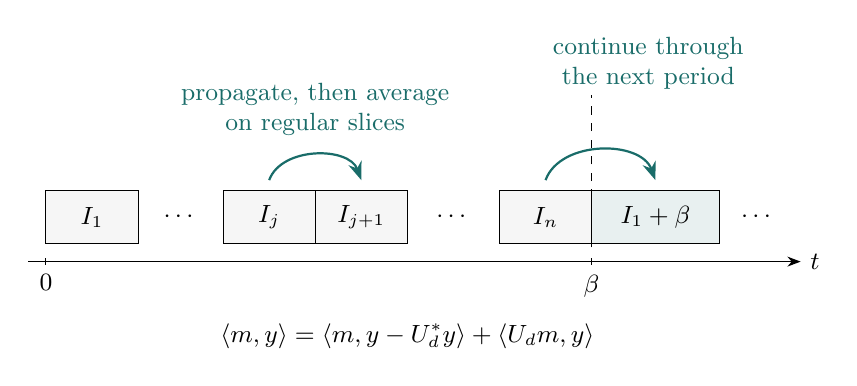
\begin{tikzpicture}[x=0.9cm,y=0.9cm,>=Stealth,
 every node/.style={font=\small}]
 \definecolor{flowblue}{RGB}{25,108,105}
 \foreach \a/\b/\lab in {0/1.3/I_1,2.5/3.8/I_j,3.8/5.1/I_{j+1},6.4/7.7/I_n}
  {\draw[fill=gray!7] (\a,0) rectangle (\b,0.75);
   \node at ({(\a+\b)/2},0.375) {$\lab$};}
 \node at (1.9,0.375) {$\cdots$};
 \node at (5.75,0.375) {$\cdots$};
 \draw[fill=flowblue!10] (7.7,0) rectangle (9.5,0.75);
 \node at (8.6,0.375) {$I_1+\beta$};
 \node at (10.05,0.375) {$\cdots$};
 \draw[->] (-0.25,-0.25)--(10.65,-0.25) node[right] {$t$};
 \draw (0,-0.2)--(0,-0.3) node[below] {$0$};
 \draw (7.7,-0.2)--(7.7,-0.3) node[below] {$\beta$};
 \draw[dashed] (7.7,-0.05)--(7.7,2.1);
 \draw[->,thick,flowblue] (3.15,0.9) to[out=70,in=110] (4.45,0.9);
 \node[align=center,text=flowblue] at (3.8,1.9) {propagate, then average\\on regular slices};
 \draw[->,thick,flowblue] (7.05,0.9) to[out=70,in=110] (8.6,0.9);
 \node[align=center,text=flowblue] at (8.5,2.55) {continue through\\the next period};
 \node[align=center] at (5.1,-1.3)
  {$\langle m,y\rangle=\langle m,y-U_d^*y\rangle+\langle U_dm,y\rangle$};
\end{tikzpicture}
\caption{Averaging the source mass from one block in the next block.
The last block uses the first block of a copied period. The displayed identity
separates the pairing of its terminal mass $m$ into a term controlled by contraction energy
and a term whose propagation can be split at the copied averaging slices.
The averaging windows are disjoint modulo one period, so their Dirichlet
energies are summed with a constant total cost. Block widths are schematic.}
\label{fig:period-averaging}
\end{figure}


For each \(j\), average over the fully regular subset of its
successor block.  Proposition~\ref{prop:good} gives this subset
measure at least \(cL\).  Applying Cauchy--Schwarz in that time
variable bounds its averaged localized pairing by
\begin{equation}\label{eq:blockaverage}
 C\sqrt{F_j/L}
 \left(\int_{I_{j+1}}\D_t(Y_j(t))\,dt\right)^{1/2},
\end{equation}
where \(Y_j(t)=T_{\beta,t}^*y\) for \(j<n\), whereas
\(Y_n(t)=T_{2\beta,t}^*y\) and \(I_{n+1}=\beta+I_1\).
The intervals \(I_2,\ldots,I_n\) are disjoint in the original
period, and \(\beta+I_1\) lies in the copied period.  Each full
period has the bound \eqref{eq:energy-suffix}, so
\[
 \sum_{j=1}^n\int_{I_{j+1}}\D_t(Y_j(t))\,dt\le2e_y.
\]
Cauchy--Schwarz across the block indices in
\eqref{eq:blockaverage}, followed by \eqref{eq:lastblockcorrection},
gives
\begin{equation}\label{eq:smoothdualcoefficient}
 \left|\sum_{j=1}^n\ip{m_j}{y}\right|
 \le C\left(\sum_{j=1}^nF_j/L+K_n\right)^{1/2}\sqrt{e_y}
       +C_0\rho(\beta).
\end{equation}
The sum of localization errors is still rapidly small because
\(n\le C\beta/L\).

The expectation of the first term in parentheses is bounded by
\(C\beta/L^2\) times the right side of
\eqref{eq:blockflowexpectation}.  Substituting
\(\lambda=\beta^{-3/2}\), \(D_*=\sqrt\beta\), and
\(b_*=\beta^{-1}R^{-3}\), this is
\begin{equation}\label{eq:smoothdualexpectation}
 C\left[
 L^4\beta^{-3}
 +L^{-1/2}\beta^{-4}R
 +L^3\beta^{-11/2}R
 +\frac1{\beta R}\right].
\end{equation}
Likewise, \eqref{eq:lastblocknorm} and the one-point snapshot bound
give
\begin{equation}\label{eq:copycorrectionexpectation}
 \EE_P[\ind_{\mathcal G}K_n]
 \le C\left(L^5\beta^{-4}+L^5\beta^{-2}R^{-3}\right).
\end{equation}
Thus the block argument has converted cancellation of source mass
into a dual energy bound.  It remains to handle the early
point-profile sources, for which cancellation at the scale \(L\)
was not used.

\subsection{Early point-profile sources}

\begin{lemma}[Diffusion of the early sources]\label{lem:earlysourceenergy}
Let \(\mu_d^{\mathrm{early}}\) be the terminal mass of the
point-profile obstacle sources at elapsed times in \([0,\beta/2)\),
and let \(M\) be their total variation before propagation.  Then
\begin{equation}\label{eq:earlymassmoment}
 \EE_P[\ind_{\mathcal G}M^2]\le H_\beta\beta^{-3/2}.
\end{equation}
For every test vector of Proposition~\ref{prop:dualenergy}, on
\(\mathcal G\),
\begin{equation}\label{eq:earlydualbound}
 \abs{\ip{\mu_d^{\mathrm{early}}}{y}}
 \le CM\beta^{-3/4}\sqrt{e_y}+C_0\rho(\beta).
\end{equation}
\end{lemma}

\begin{proof}
For a bin beginning at elapsed time \(s\), put
\(d_s=\sqrt{1+s}\).  Lemma~\ref{lem:sourcebins} bounds its source
variation on \(\mathcal G\) by
\(H_\beta\sum_\alpha W_{d_s}(z_\alpha)\), where the sum is over
the obstacle slots above \(B_{4R}(x)\) at that bin's starting slice.
The single-box
case of Lemma~\ref{lem:boxmoment} gives
\begin{align*}
 \left\|\sum_\alpha W_{d_s}(z_\alpha)\right\|_{L^2(\PP_P)}
 &\le C\left(\sqrt\lambda\,\norm{W_{d_s}}_2
                +\lambda\norm{W_{d_s}}_1\right)\\
 &\le C\left(\beta^{-3/4}d_s^{-5/2}
                 +\beta^{-3/2}d_s^{-1}\right)=J(d_s).
\end{align*}
Minkowski's inequality in the probability space now gives
\[
 \|\ind_{\mathcal G}M\|_{L^2(\PP_P)}
 \le H_\beta\sum_{\mathrm{bins}}J(d_s)
 \le H_\beta\beta^{-3/4}.
\]
For the last inequality, bins have lengths between \(1\) and \(3\),
so the sum of \(d_s^{-5/2}=(1+s)^{-5/4}\) is bounded and the sum of
\(d_s^{-1}=(1+s)^{-1/2}\) is at most \(C\sqrt\beta\).
Absorbing the square of a logarithmic factor into \(H_\beta\)
proves \eqref{eq:earlymassmoment}.  This use of Minkowski requires
no independence of the bin snapshots.

Propagate all these sources to a slice in a block contained in the
last quarter of the traversal.  Every propagation has elapsed time
at least \(\beta/4\).  Localize to \(B_{6R}(x)\); by
Lemma~\ref{lem:localization}, the discarded total variation is
rapidly small on \(\mathcal G\).  Lemma~\ref{lem:heatbound}
and substochasticity show that a localized unit point mass has total
mass at most one and maximum entry at most \(C\beta^{-3/2}\).
The additional spatial restriction only decreases the kernel.
Consequently the localized signed source mass \(\nu_t\) is
dominated in absolute value by a nonnegative mass \(\sigma_t\)
such that
\[
 \norm{\sigma_t}_1\le M,
 \qquad
 \norm{\sigma_t}_\infty\le CM\beta^{-3/2}.
\]

At a fully regular such slice, use the unit flows of
Lemma~\ref{lem:flowoverlap}.  For every slot \(a\), splitting
distances at \(D_*\) gives
\begin{align*}
 \sum_{a'}\frac{\sigma_t(a')}{1+\dist(a,a')}
 &\le CM\beta^{-3/2}D_*^2+CM D_*^{-1}\\
 &\le CM\beta^{-1/2}.
\end{align*}
Superposing the unit flows with coefficients \(\nu_t(a)\) therefore
gives a flow with divergence \(\nu_t\) and squared norm at most
\[
 C\sum_{a,a'}\frac{\sigma_t(a)\sigma_t(a')}
                         {1+\dist(a,a')}
 \le CM^2\beta^{-1/2}.
\]
There are blocks of total length at least \(c\beta\) contained
in the last quarter, and at least half of each is fully regular.
Average \eqref{eq:flowpairing-energy} over this regular set.
Cauchy--Schwarz in time and \eqref{eq:energy-suffix} give
\eqref{eq:earlydualbound}.
\end{proof}

\begin{proof}[Proof of Proposition~\ref{prop:dualenergy}]
The two collections exhaust the sources in the chosen direction.
Combine \eqref{eq:smoothdualcoefficient} and
\eqref{eq:earlydualbound}, and choose a measurable coefficient with
\[
 X_d^2\le C\left(\sum_{j=1}^nF_j/L+K_n+M^2\beta^{-3/2}\right).
\]
All expressions on the right are measurable functions of the
exposure; none depends on the test vector.  Equations
\eqref{eq:smoothdualexpectation},
\eqref{eq:copycorrectionexpectation}, and
\eqref{eq:earlymassmoment} bound its expectation on
\(\mathcal G\).  With \(L=\beta^\delta\) and
\(R=\beta^{3/2+\delta/4}\), their sum is at most
\begin{equation}\label{eq:energyfinalpowers}
 C\left[
 \beta^{-3+4\delta}
 +\beta^{-5/2-\delta/4}
 +\beta^{-4+13\delta/4}
 +\beta^{-4+5\delta}
 +\beta^{-13/2+17\delta/4}
 +H_\beta\beta^{-3}\right]
 =o(\beta^{-5/2}),
\end{equation}
since \(\delta=1/200\).
The term \(\beta^{-5/2-\delta/4}\) covers both the isolated
net-mass flows and the cutoff flows.  All localization errors were
estimated in \(\ell^1\) against test vectors of supremum norm
at most a constant times \(C_0\), so they give the uniform
rapidly small remainder in \eqref{eq:dualenergy}.
The argument used elapsed time and the ordered kernels throughout;
it applies to \(U\) and to \(U^*\) with the same bounds.
Adding the two expected squares proves
\eqref{eq:dualenergyexpectation}.
\end{proof}

\section{From the pinned comparison to magnetization}\label{sec:pressure}

We first combine the two residual estimates to prove the uniform
pinned comparison.  We then express a positive field as a mixture
of deterministic pin sets.  Integrating the finite-volume
magnetization bounds in the field will preserve the required order:
volume tends to infinity before the field tends to zero.

\subsection{Completion of the capacity comparison}

\begin{proof}[Proof of Proposition~\ref{prop:comparison}]
Fix the cube, pins, and starting slot in the proposition, and expose
the cycles under $\PP_P$, $P=E\cup\{i\}$.
Use the trial vector $h$ and constant $c$ from
\eqref{eq:trialvector} and \eqref{eq:freepotential}.
On the good event $\mathcal G$ of Proposition~\ref{prop:good},
Proposition~\ref{prop:dualenergy}, applied with a fixed supremum
bound $2$, gives a measurable $X$ such that
\[
 \abs{\ip{\mu_d}{z}}\le X\sqrt{e_z}+\varepsilon_\beta,
 \qquad d=+,-,
\]
for vectors vanishing on killed cut slots with
$\norm{z}_\infty\le2$, where $\varepsilon_\beta$ is rapidly small
and
\[
 \EE_P[\ind_{\mathcal G}X^2]=o(\beta^{-5/2}).
\]
If the two directions initially give different coefficients, take
their maximum; this preserves the displayed expectation bound.
The source identities \eqref{eq:residualdefinition} identify these
residuals with those in \eqref{eq:capacityresiduals}.
Since $0\le h\le1$, the averaged capacity criterion
\eqref{eq:averagedcapacity} applies.  Proposition~\ref{prop:scalar}
and the probability estimate in Proposition~\ref{prop:good} give
\begin{equation}\label{eq:returncomparison}
 r:=\EE_Pq_i=1-c+o(\beta^{-5/2}).
\end{equation}
Every error here is uniform over the cube and the allowed pin sets.
In particular, the good-event estimate is used only through its
probability on the complement; there $q_i\in[0,1]$ suffices.

By Lemma~\ref{lem:freebounds}, $v(x)=O(\beta^{-3/2})$, so
\[
 1-c=\frac{v(x)}{1+v(x)}=v(x)+O(\beta^{-3}).
\]
The exact pin identity \eqref{eq:pinreturn} now yields
\begin{equation}\label{eq:slotcomparison}
 d_E(i)=\frac{r}{1+r}
       =v(x)+o(\beta^{-5/2})
       =\frac1\ell\sum_{n\ge1}p_{n\beta}(0)
          +o(\beta^{-5/2}).
\end{equation}
Indeed $r=O(\beta^{-3/2})$, so the second rational transformation
also costs only $O(\beta^{-3})$.
By \eqref{eq:freeidealdensity}, the last sum is
$n_S^{\rm sw}(\beta)$.  The uniform little-oh
in \eqref{eq:slotcomparison} is equivalent to the asserted function
$\varepsilon_S(\beta)\to0$ after choosing a sufficiently large
$\beta_0(S)$.  Equations \eqref{eq:returncomparison} and
\eqref{eq:freeidealdensity}, together with
$1-c=v(x)+O(\beta^{-3})$, also give
$r=\ell^{-1}n_S^{\rm sw}(\beta)+o(\beta^{-5/2})$, as asserted.
\end{proof}

\subsection{Boundary pins and field pins}

Write $V_N=|\Lambda_N|$, use
$\partial\Lambda_N=\partial_{\mathrm{in}}\Lambda_N$ for the inner
boundary, and let $q_{\Lambda_N}$ be the number of slot edges.
For a picture $\omega$, let $\mathcal C(\omega)$ be
its cycles and $a_C$ the number of time-zero slots on $C$.
For colors $\sigma_C\in\{-1,1\}$, define
\[
 M(\omega,\sigma)=\frac12\sum_Ca_C\sigma_C,
 \qquad
 N_\downarrow(\omega,\sigma)=\sum_{C:\,\sigma_C=-1}a_C
                              =SV_N-M(\omega,\sigma).
\]
Let $\chi_D(\omega,\sigma)$ indicate that every cycle meeting $D$
is up.  The spin-loop representation in
Proposition~\ref{prop:loopinputs} identifies the ordinary partition
function with
\[
 Z_N(t)=e^{\beta q_{\Lambda_N}/4}
       \EE_{\rm b}\sum_\sigma e^{\beta tM(\omega,\sigma)},
 \qquad p_N(t)=\frac{\log Z_N(t)}{\beta V_N}.
\]
Its boundary-pinned counterpart and pressure are
\begin{equation}\label{eq:pinnedpressure}
 Z_N^+(t)=e^{\beta q_{\Lambda_N}/4}
       \EE_{\rm b}\sum_\sigma
          \chi_{D_0}(\omega,\sigma)e^{\beta tM(\omega,\sigma)},
 \qquad
 p_N^+(t)=\frac{\log Z_N^+(t)}{\beta V_N}.
\end{equation}

We use the surface estimate of
\cite[Proposition~7.1]{BlochLaw}.  Its argument is short and records why
all-times boundary pins do not change the pressure.

\begin{lemma}[Surface cost of boundary pins]\label{lem:surfacecost}
For every finite $\beta>0$, every $t\ge0$, and every finite cube,
\begin{equation}\label{eq:surfacecost}
 0\le p_N(t)-p_N^+(t)
 \le (\log2)\left(\frac\ell\beta+24\ell^2\right)
        \frac{|\partial\Lambda_N|}{V_N}.
\end{equation}
In particular $p_N^+(t)\to p_{S,\beta}(t)$ for each fixed
$\beta>0$ and $t\ge0$.
\end{lemma}

\begin{proof}
After extracting the all-up factor, the field-tilted picture weight is
\[
 W_t(\omega)=\prod_C(1+e^{-\beta t a_C}).
\]
Let $\EE_t$ denote expectation under this tilted picture law.
Given the picture, each cycle is up independently with probability
$(1+e^{-\beta t a_C})^{-1}\ge1/2$.  If $b_0$ counts cycles meeting
$D_0$, Jensen's inequality therefore gives
\[
 1\ge\frac{Z_N^+(t)}{Z_N(t)}
   \ge\EE_t2^{-b_0}
   \ge\exp[-(\log2)\EE_t b_0].
\]
Let $J_\partial$ count marks on slot edges incident to a boundary
site, and let $q_\partial$ be the number of those edges.
Every boundary-meeting cycle either has a boundary slot at time zero
or passes through one of these marks.  A mark belongs to at most two
cycles, so
\[
 b_0\le\ell|\partial\Lambda_N|+2J_\partial,
 \qquad q_\partial\le6\ell^2|\partial\Lambda_N|.
\]
Insertion of one mark joins two cycles or splits one.  Each factor
of $W_t$ lies in $[1,2]$, and at most two new factors appear, whence
$W_t(\omega\cup\{u\})\le4W_t(\omega)$ for almost every inserted
mark $u$.  The Poisson insertion formula at rate $1/2$ implies
\[
 \EE_t J_\partial\le2\beta q_\partial
               \le12\beta\ell^2|\partial\Lambda_N|.
\]
The preceding inequalities, divided by $\beta V_N$, prove
\eqref{eq:surfacecost}.  The pressure limit follows because the
boundary-to-volume ratio tends to zero.
\end{proof}

For $t\ge0$ put $b_\beta(t)=1-e^{-\beta t}$, and let $\nu_b$
be the law that selects each time-zero slot independently with
probability $b=b_\beta(t)$.  If $A$ is the selected set and
$\operatorname{Up}(\omega,\sigma)$ is the set of up slots at that
cut, then
\begin{equation}\label{eq:fieldpinidentity}
 \sum_A\nu_b(A)\ind_{\{A\subset\operatorname{Up}\}}
   =(1-b)^{N_\downarrow}=e^{-\beta tN_\downarrow}.
\end{equation}
Consequently the field law in \eqref{eq:pinnedpressure} is the
picture/color marginal of the joint law
\begin{equation}\label{eq:fieldjointlaw}
 \widehat\PP_{N,t}(d\omega,d\sigma,A)
  \ \propto\ \PP_{\rm b}(d\omega)\,\nu_b(A)
                         \chi_{D_0\cup A}(\omega,\sigma),
\end{equation}
where the color variable uses counting measure.
Indeed the common factor extracted from its normalizer is
$e^{\beta q_{\Lambda_N}/4+\beta tSV_N}$.
Conditional on $A$, this is exactly the zero-field color law with
the deterministic pins $E=D_0\cup A$.

The marginal law of $A$ is generally not Bernoulli, because its
normalization is weighted by the pinned partition function.
Conditioning instead on $(\omega,\sigma)$ makes selections on up
slots independent Bernoulli choices of parameter $b$, and forbids
selections on down slots.  Thus every specified slot $j$ satisfies
\begin{equation}\label{eq:fieldpinbound}
 \widehat\PP_{N,t}(j\in A)
   =b_\beta(t)\widehat\PP_{N,t}(j\text{ up})\le b_\beta(t).
\end{equation}
This is the only property of the posterior pin law needed below.

\subsection{Thermodynamic and zero-field limits}

\begin{proof}[Proof of Theorem~\ref{thm:main}]
Fix $S$ and a sufficiently large $\beta$.  The finite-volume
magnetization is bounded, so differentiation under the sum in
\eqref{eq:pinnedpressure} is justified.  Equations
\eqref{eq:fieldjointlaw} and \eqref{eq:fieldpinidentity} give
\begin{equation}\label{eq:pressuredeficit}
 S-(p_N^+)'(t)
  =\frac1{V_N}\widehat\EE_{N,t}N_\downarrow
 =\frac1{V_N}\sum_{j\text{ at time }0}
                         \widehat\EE_{N,t}d_{D_0\cup A}(j).
\end{equation}
Here $d_E(j)$ means the down probability also for pinned slots, where
it is zero.
Let $\rho_N$ be the fraction of sites $x$ for which
$B_{50R_*}(x)$ is interior to $\Lambda_N$.
For such a site let $\mathcal A_x$ be the event that no selected
pin lies above that ball.  A union bound using
\eqref{eq:fieldpinbound} gives
\[
 \widehat\PP_{N,t}(\mathcal A_x^c)
 \le C_{S,\beta}\,b_\beta(t),
\]
where $C_{S,\beta}$ is finite and independent of $N$.
On $\mathcal A_x$, Proposition~\ref{prop:comparison} applies to
each of the $\ell$ slots at $x$, for every conditional pin set $A$.
On its complement, and at sites outside the interior region, use
the boundedness of down probabilities.  Summing the slot estimates
in \eqref{eq:pressuredeficit} gives
\begin{equation}\label{eq:derivativecomparison}
 \abs{S-(p_N^+)'(t)-n_S^{\rm sw}(\beta)}
 \le \ell\varepsilon_S(\beta)\beta^{-5/2}
       +C_S(1-\rho_N)+C_{S,\beta}b_\beta(t).
\end{equation}
Here $n_S^{\rm sw}(\beta)$ is bounded for the large values of $\beta$
under consideration, so its contribution on exceptional
sites is included in $C_S$.

Integrate \eqref{eq:derivativecomparison} over $t\in[0,h]$, for
$h>0$, and divide by $h$.  Now take $N\to\infty$, keeping
$\beta$ and $h$ fixed.  The radius is fixed in this limit, so
$\rho_N\to1$, and Lemma~\ref{lem:surfacecost} gives convergence
of $p_N^+$ at both field endpoints.  We obtain
\[
 \abs{S-\frac{p_{S,\beta}(h)-p_{S,\beta}(0)}h
                    -n_S^{\rm sw}(\beta)}
 \le \ell\varepsilon_S(\beta)\beta^{-5/2}
       +\frac{C_{S,\beta}}h\int_0^h b_\beta(t)\,dt.
\]
For this fixed $\beta$, the last term tends to zero as
$h\downarrow0$.  Convexity and the uniform magnetization bound
give the right derivative of the limiting pressure.  Therefore
\[
 \abs{S-m_S(\beta)-n_S^{\rm sw}(\beta)}
 \le\ell\varepsilon_S(\beta)\beta^{-5/2}.
\]
Finally let $\beta\to\infty$.  Since $S$ is fixed, multiplication
by $(\beta S)^{5/2}$ proves the theorem.
\end{proof}

\subsection{The explicit lattice correction}

The full ideal density has a two-term expansion with a remainder
small enough to identify the coefficient in
Corollary~\ref{cor:expansion}.

\begin{proof}[Proof of Corollary~\ref{cor:expansion}]
Put $t=\beta S$.  Independence of the three coordinates gives
\[
 p_\beta(0)=I(t)^3,\qquad
 I(t)=\frac1{2\pi}\int_{-\pi}^{\pi}
                         e^{-2t(1-\cos k)}\,dk.
\]
We claim, uniformly for $t\ge1$, that
\begin{equation}\label{eq:laplaceexpansion}
 I(t)=\frac1{\sqrt{4\pi t}}
          \left(1+\frac1{16t}+O(t^{-2})\right).
\end{equation}
To see this, set $u=\sqrt t\,k$ and first restrict to
$|u|\le t^{1/10}$.  Taylor's formula gives
\[
 2t(1-\cos(u/\sqrt t))
       =u^2-\frac{u^4}{12t}+O(u^6/t^2),
\]
and hence, on this interval,
\[
 e^{-2t(1-\cos(u/\sqrt t))}
 =e^{-u^2}\left(1+\frac{u^4}{12t}
                   +O\!\left(\frac{u^6+u^8}{t^2}\right)\right).
\]
The bound $2(1-\cos k)\ge c k^2$ controls the omitted interval by
$O(e^{-c t^{1/5}})$ after the same rescaling.  Extending the
Gaussian integrals to $\R$ has an error of this size as well.
Since
\[
 \int_\R e^{-u^2}\,du=\sqrt\pi,
 \qquad
 \int_\R u^4e^{-u^2}\,du=\frac34\sqrt\pi,
\]
the formula \eqref{eq:laplaceexpansion} follows, with a constant
that can be enlarged to cover all $t\ge1$.
Cubing gives
\[
 p_\beta(0)
   =(4\pi t)^{-3/2}\left(1+\frac3{16t}+O(t^{-2})\right).
\]
Apply this uniform estimate at $nt$, $n\ge1$, and sum.
The remainder is bounded by
$Ct^{-7/2}\sum_{n\ge1}n^{-7/2}$, so
\begin{equation}\label{eq:idealdensityexpansion}
 n_S^{\rm sw}(\beta)
  =\frac{\zeta(3/2)}{8\pi^{3/2}}(\beta S)^{-3/2}
   +\frac{3\zeta(5/2)}{128\pi^{3/2}}(\beta S)^{-5/2}
   +O((\beta S)^{-7/2}).
\end{equation}
Theorem~\ref{thm:main} now gives the asserted expansion of
$S-m_S(\beta)$.
\end{proof}

\begin{thebibliography}{99}

\bibitem{Benedikter2017}
N.~Benedikter.
Interaction corrections to spin-wave theory in the large-\(S\) limit of the
quantum Heisenberg ferromagnet.
\emph{Mathematical Physics, Analysis and Geometry} \textbf{20} (2017), article~5.
\href{https://doi.org/10.1007/s11040-016-9237-6}{doi:10.1007/s11040-016-9237-6}.

\bibitem{Bloch1930}
F.~Bloch.
Zur Theorie des Ferromagnetismus.
\emph{Zeitschrift f\"ur Physik} \textbf{61} (1930), 206--219.
\href{https://doi.org/10.1007/BF01339661}{doi:10.1007/BF01339661}.

\bibitem{ConlonSolovej1991}
J.~G.~Conlon and J.~P.~Solovej.
Upper bound on the free energy of the spin \(1/2\) Heisenberg ferromagnet.
\emph{Letters in Mathematical Physics} \textbf{23} (1991), 223--231.
\href{https://doi.org/10.1007/BF01885500}{doi:10.1007/BF01885500}.

\bibitem{CGS2015}
M.~Correggi, A.~Giuliani, and R.~Seiringer.
Validity of the spin-wave approximation for the free energy of the
Heisenberg ferromagnet.
\emph{Communications in Mathematical Physics} \textbf{339} (2015), 279--307.
\href{https://doi.org/10.1007/s00220-015-2402-0}{doi:10.1007/s00220-015-2402-0}.

\bibitem{Dyson1956a}
F.~J.~Dyson.
General theory of spin-wave interactions.
\emph{Physical Review} \textbf{102} (1956), 1217--1230.
\href{https://doi.org/10.1103/PhysRev.102.1217}{doi:10.1103/PhysRev.102.1217}.

\bibitem{Dyson1956b}
F.~J.~Dyson.
Thermodynamic behavior of an ideal ferromagnet.
\emph{Physical Review} \textbf{102} (1956), 1230--1244.
\href{https://doi.org/10.1103/PhysRev.102.1230}{doi:10.1103/PhysRev.102.1230}.

\bibitem{GaudilliereLandim2014}
A.~Gaudilli\`ere and C.~Landim.
A Dirichlet principle for non reversible Markov chains and some recurrence
theorems.
\emph{Probability Theory and Related Fields} \textbf{158} (2014), 55--89.
\href{https://doi.org/10.1007/s00440-012-0477-5}{doi:10.1007/s00440-012-0477-5}.
Author preprint:
\href{https://arxiv.org/abs/1111.2445v1}{arXiv:1111.2445v1}.

\bibitem{Hofmann2017}
C.~P.~Hofmann.
Cubic ideal ferromagnets at low temperature and weak magnetic field.
\emph{Physica B: Condensed Matter} \textbf{510} (2017), 117--126.
\href{https://doi.org/10.1016/j.physb.2017.01.019}{doi:10.1016/j.physb.2017.01.019}.

\bibitem{HolsteinPrimakoff1940}
T.~Holstein and H.~Primakoff.
Field dependence of the intrinsic domain magnetization of a ferromagnet.
\emph{Physical Review} \textbf{58} (1940), 1098--1113.
\href{https://doi.org/10.1103/PhysRev.58.1098}{doi:10.1103/PhysRev.58.1098}.

\bibitem{Nachtergaele1994}
B.~Nachtergaele.
Quasi-state decompositions for quantum spin systems.
In B.~Grigelionis et al. (eds.),
\emph{Probability Theory and Mathematical Statistics},
Proceedings of the Sixth Vilnius Conference,
VSP/TEV, Utrecht--Tokyo--Vilnius, 1994, pp.~565--590.
\href{https://arxiv.org/abs/cond-mat/9312012v2}{arXiv:cond-mat/9312012v2}.

\bibitem{Nash1958}
J.~Nash.
Continuity of solutions of parabolic and elliptic equations.
\emph{American Journal of Mathematics} \textbf{80} (1958), 931--954.
\href{https://doi.org/10.2307/2372841}{doi:10.2307/2372841}.

\bibitem{BlochLaw}
OpenAI.
\emph{Bloch's Law for Finite-Range Heisenberg Ferromagnets in Three Dimensions}.
OpenAI Math Release preprint
\href{https://github.com/openai/math/blob/main/preprints/Blochs-Law-for-Finite-Range-Heisenberg-Ferromagnets-in-Three-Dimensions-October-5-2026/bloch-law-heisenberg.pdf}{OAI:Blochs-Law-for-Finite-Range-Heisenberg-Ferromagnets-in-Three-Dimensions-October-5-2026},
2026.

\bibitem{Ordering}
OpenAI.
\emph{Spontaneous magnetization in the quantum Heisenberg ferromagnet}.
OpenAI Math Release preprint
\href{https://github.com/openai/math/blob/main/preprints/Spontaneous-magnetization-in-the-quantum-Heisenberg-ferromagnet-September-24-2026/paper.pdf}{OAI:Spontaneous-magnetization-in-the-quantum-Heisenberg-ferromagnet-September-24-2026},
2026.

\bibitem{Toth1993}
B.~T\'oth.
Improved lower bound on the thermodynamic pressure of the spin \(1/2\)
Heisenberg ferromagnet.
\emph{Letters in Mathematical Physics} \textbf{28} (1993), 75--84.
\href{https://doi.org/10.1007/BF00739568}{doi:10.1007/BF00739568}.

\end{thebibliography}

\end{document}
